\documentclass[12pt]{article}
%\usepackage[utf8]{inputenc}
%\documentclass[UTF8]{ctexart}
%\usepackage[UTF8, heading = false, scheme = plain]{ctex}
\usepackage{geometry}
%geometry{a4paper,scale=0.9}
\geometry{a4paper,left=1cm,right=1cm,top=1cm,bottom=2cm}
\usepackage{amsfonts}
\usepackage{color}
\usepackage{url}
%\usepackage{biblatex}
\usepackage{amsmath}
\usepackage{amssymb}
\usepackage{latexsym}
\usepackage{cite}
%\addbibresource{ref.bib}
%\bibliography{ref.bib}
\usepackage{caption}
\usepackage{graphicx, subfig}
\usepackage{float}
%\usepackage[fontset=ubuntu]{ctex}
%\usepackage{fontspec}
\usepackage{xeCJK}
%\usepackage[colorlinks,
%anchorcolor=black,
%citecolor=black]{hyperref}
%\setmainfont{SimSun}
\usepackage[section]{placeins}
\usepackage{enumitem}
\usepackage{framed}
\usepackage[framemethod=TikZ]{mdframed}
\usepackage{indentfirst}
\usepackage{setspace}%使用间距宏包
\linespread{1.5}

\title{【共享】滴滴出行业务系统的架构升级}
\author{leolinuxer}
%\date{June 2020}

\begin{document}
%\setlength{\parindent}{0pt}
\maketitle
\tableofcontents

\section{背景}
\url{https://zhuanlan.zhihu.com/p/23289547?utm_source=wechat_session&utm_medium=social&utm_oi=39537212391424}

讲师介绍:
杜欢,2015 年加入滴滴,负责公司公共业务、客户端/前端架构和新业务孵化,致力于用技术手段解决业务痛点和提升研发效率,曾作为技术负责人主导公司技术架构升级以支撑公司业务快速迭代的需求。在加入滴滴前有长达五年的创业经历,具有丰富的团队管理经验,熟悉移动互联网应用的整个技术栈。

杜欢:先自我介绍一下,我是杜欢,2015年5月加入滴滴,在此之前我有五年的创业经历,创业前曾在微软和百度任职。我非常喜欢思考一些比较抽象和有趣的东西,滴滴这样一个平台能够让我找到乐趣和兴奋点。滴滴是中国出行领域的缩影,业务非常独特,也是一个高速成长的公司。去年我考虑加入滴滴的时候,我发现有这样一个机会能够从头重新思考整个滴滴的业务形态,而且能够对它的业务产生影响,这件事情让我非常兴奋。

今天给大家主要介绍的是去年滴滴内部做的一次重大架构升级,滴滴快速发展的过程中,系统的迭代速度和其他方面的设计遇到了很多困难,这次升级就是为了解决这些困难。

去年我们做了一次非常大的重构。下图是今天要讲的大纲,我会从问题本身出发,回顾一下整个过程,包括如何发现问题、分析问题和解决方案。最后,我也会提出一些想法,如何规避重蹈这样的覆辙。

\section{挑战在哪里}
首先,我们看一下挑战在哪里。滴滴在出行领域是非常独特的公司,它的独特不在于业务模式多复杂,而在于它的发展非常快。滴滴的成立时间是2012年的6月,到现在为止才经过了四年的时间。滴滴的成长速度十分惊人,到今天它的估值已经超过260亿美元,融资轮次非常多。如果不是因为竞争非常恶劣,滴滴也不会一直用融资的方法为自己开路。在这样的压力之下,滴滴所有的动作可能都会走形,所有的想法可能因为现在一些短期利益不得不进行一些权衡。

\begin{figure}[H]
    \centering
    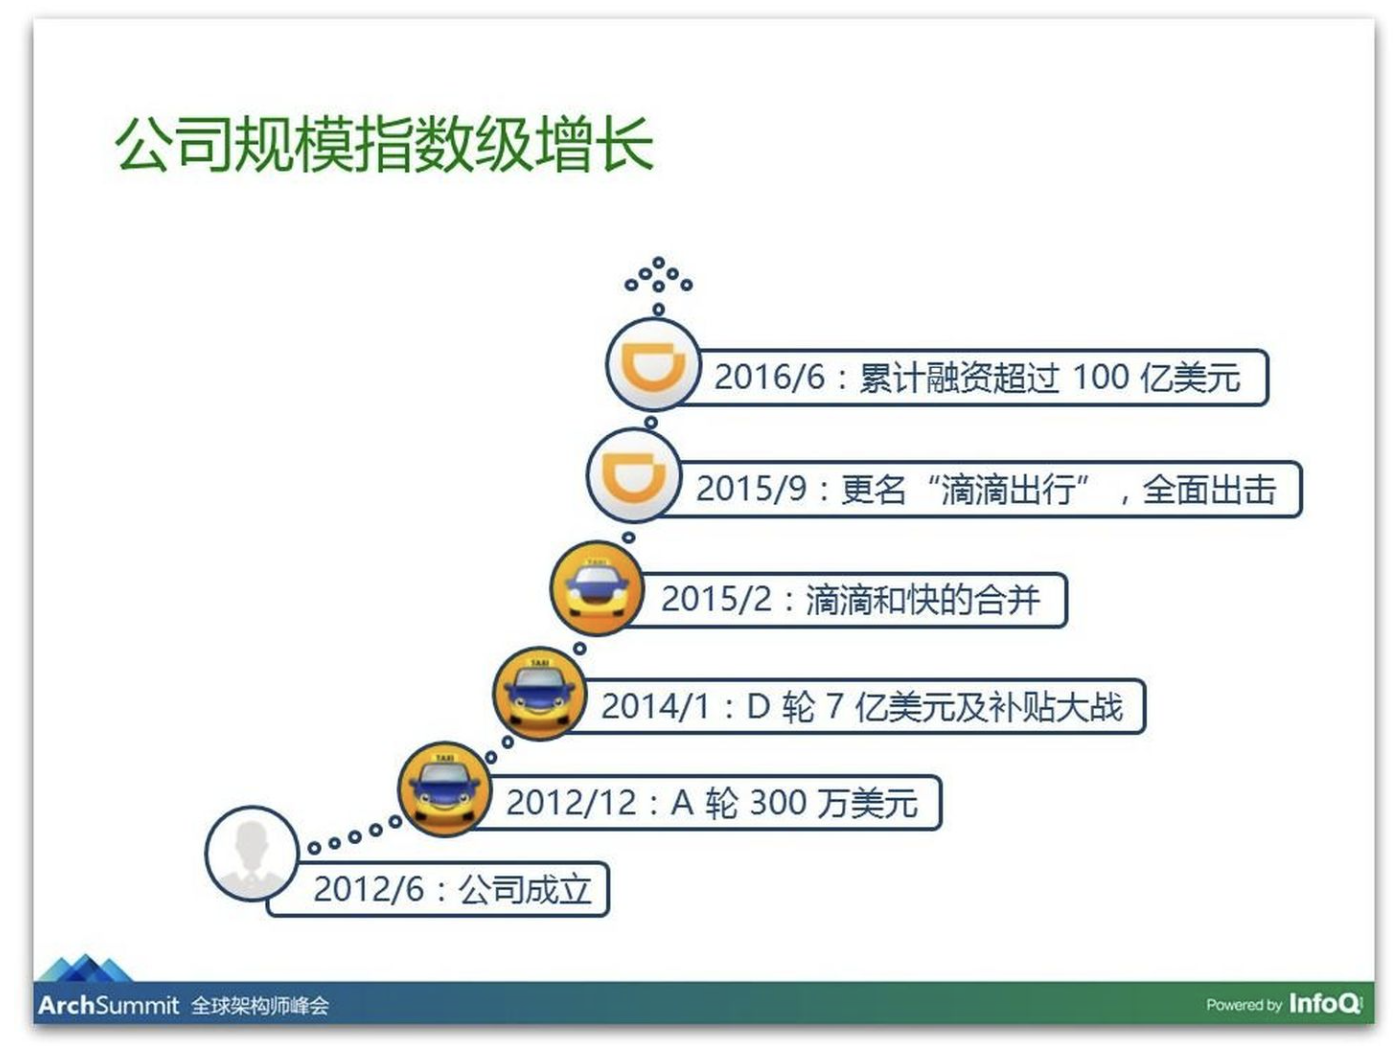
\includegraphics[width=1\textwidth]{fig/DIDI_Reconstruction_1.png}
\end{figure}

同时,公司的业务也在爆炸式地增长。如果滴滴只做一个业务,原本可以做得非常深入。滴滴从2014年开始加入了专车业务,2015年业务数量增加到七条,2016年已经超过十条。业务急速发展之中大家会思考,到底怎么做才能使这些还不稳定或者还没有想清楚的业务很好地迭代起来。想到最简单的方法是,如果新业务跟某个旧业务非常类似但又不完全一样,我们就把旧业务的旧代码复制并修改,这样新业务就做出来了。之前,这种情况经常发生,就造成了很大的问题。

\begin{figure}[H]
    \centering
    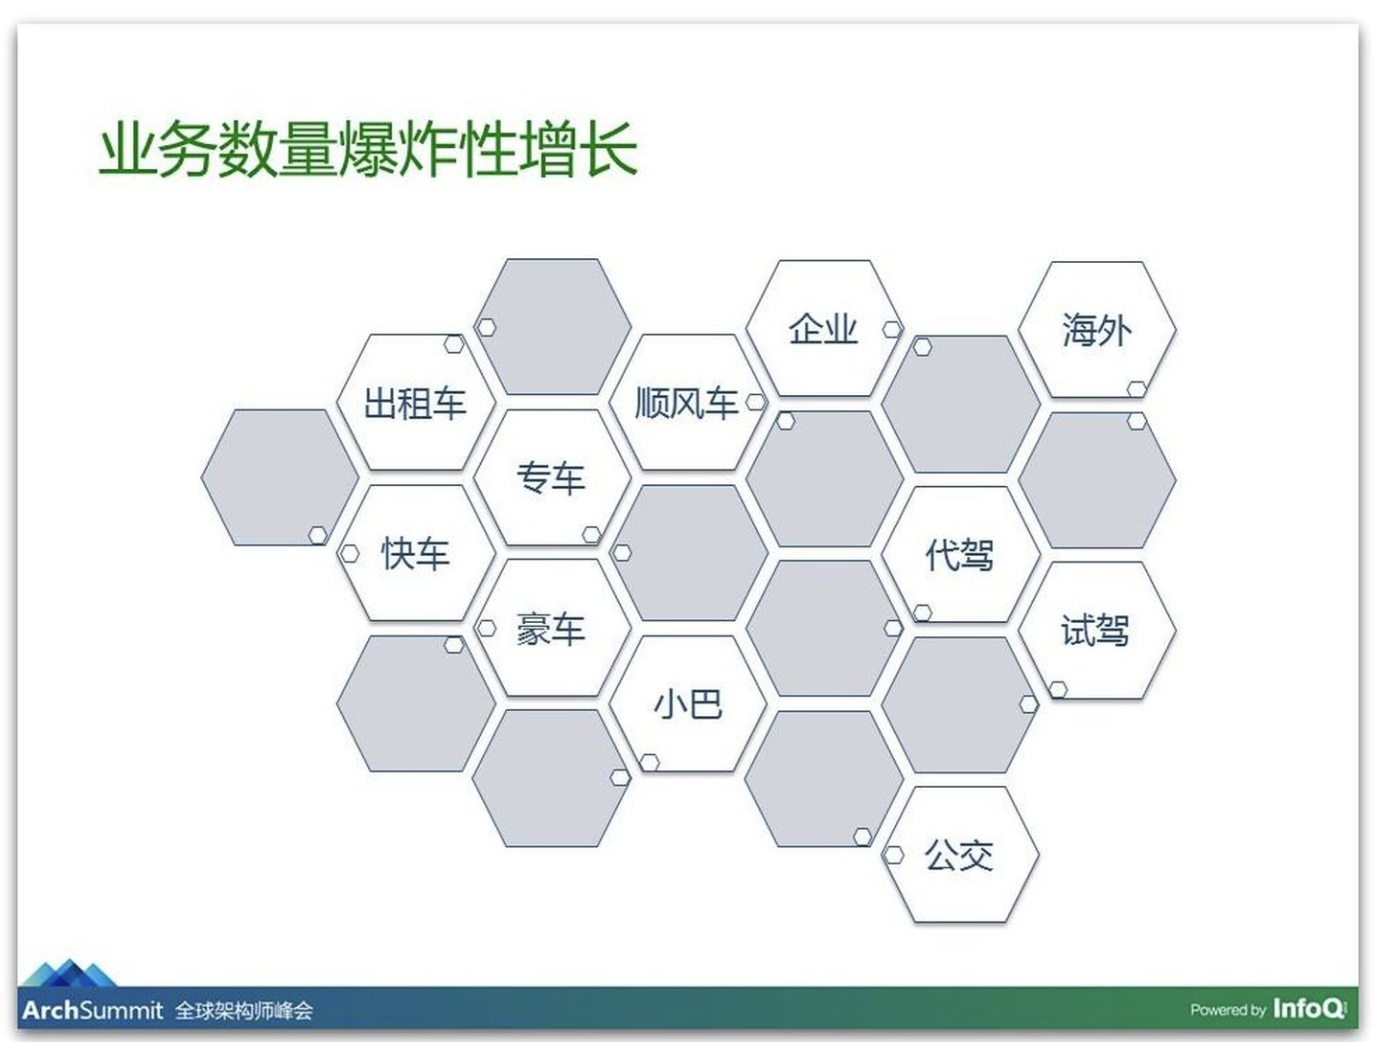
\includegraphics[width=1\textwidth]{fig/DIDI_Reconstruction_2.png}
\end{figure}

在2015年上半年,滴滴整个系统已经积累了很多问题,分布在乘客App、服务端、Web App之中。特别值得一提的是,服务端的问题并不是性能,而是在于巨大的耦合导致数据紊乱和迭代速度越来越慢。

\begin{figure}[H]
    \centering
    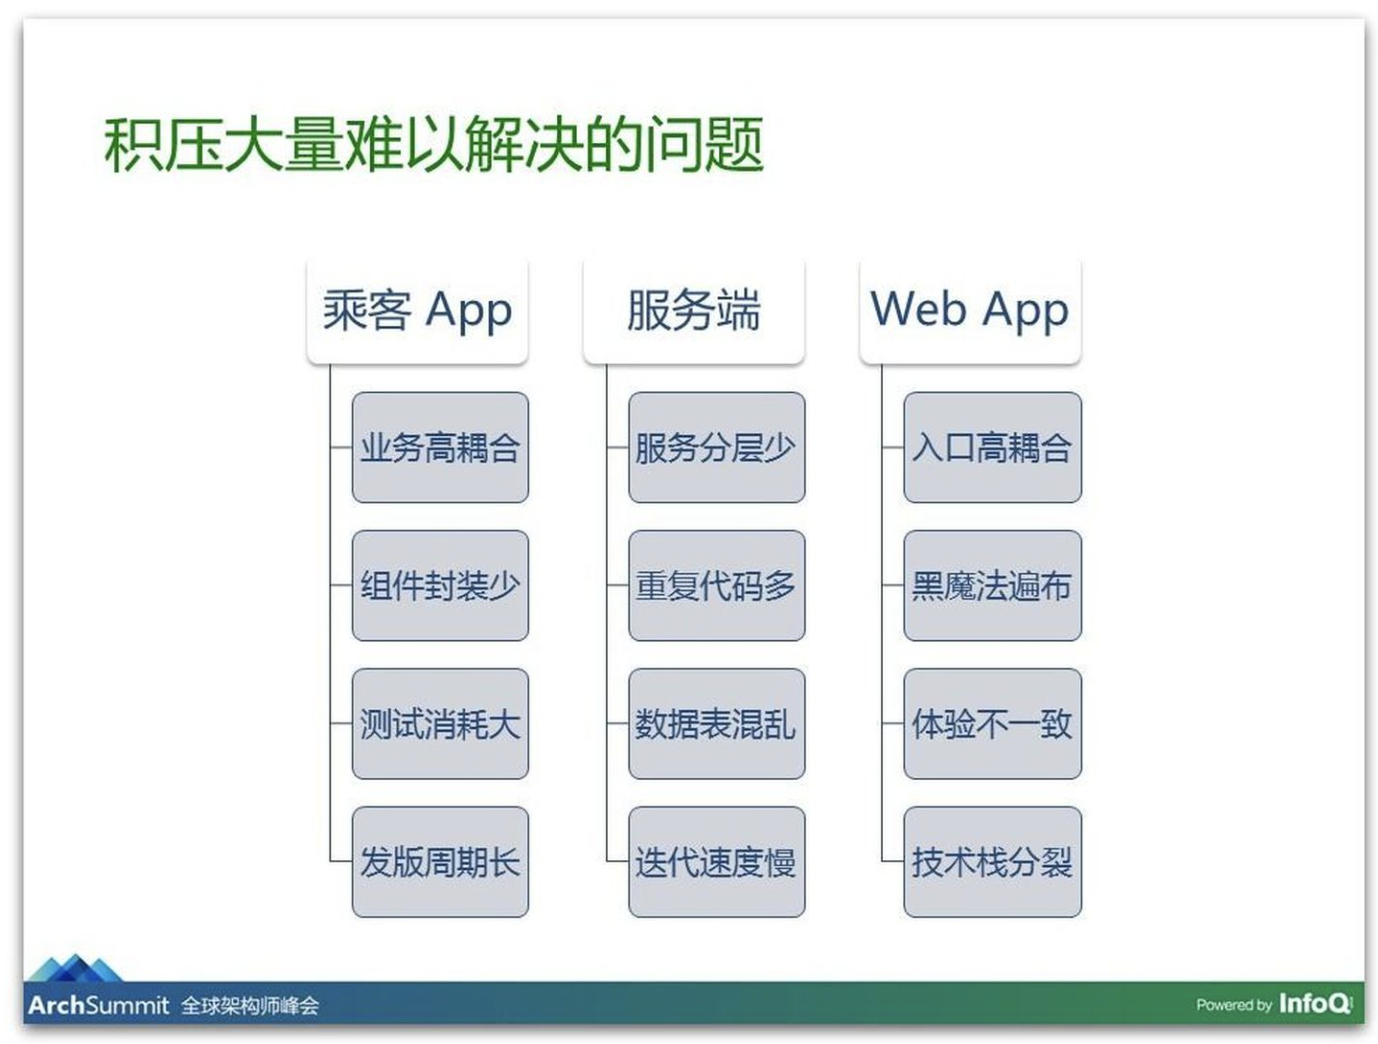
\includegraphics[width=1\textwidth]{fig/DIDI_Reconstruction_3.png}
\end{figure}

滴滴的独特性迫使我们独立思考这些问题,所有的解法都要针对滴滴现状,而不是看哪个大公司是怎么做的,然后直接复制过来。

\section{现状是什么}
在解决问题之前,我们需要了解现状是怎样的。如下图所示,在2015年下半年,滴滴的系统架构分为四层。最顶层是用户应用,每一个用户应用就是一个端,也就是用户所能看到的入口。然后是接入层,这是非常传统的结构,我们用了Nginx,还专门做了TCP接入层。在业务层,Web是非常大的集群,有非常大的代码量,我们只对业务做了分割,有策略引擎、司机调度。在数据层,有KV集群、MySQL集群、任务队列、特征存储。这是任何一个初创公司应该有的架构,我们对这个架构并没有做特殊的策划,仅仅在这个技术体系里面把业务逻辑实现出来。

\begin{figure}[H]
    \centering
    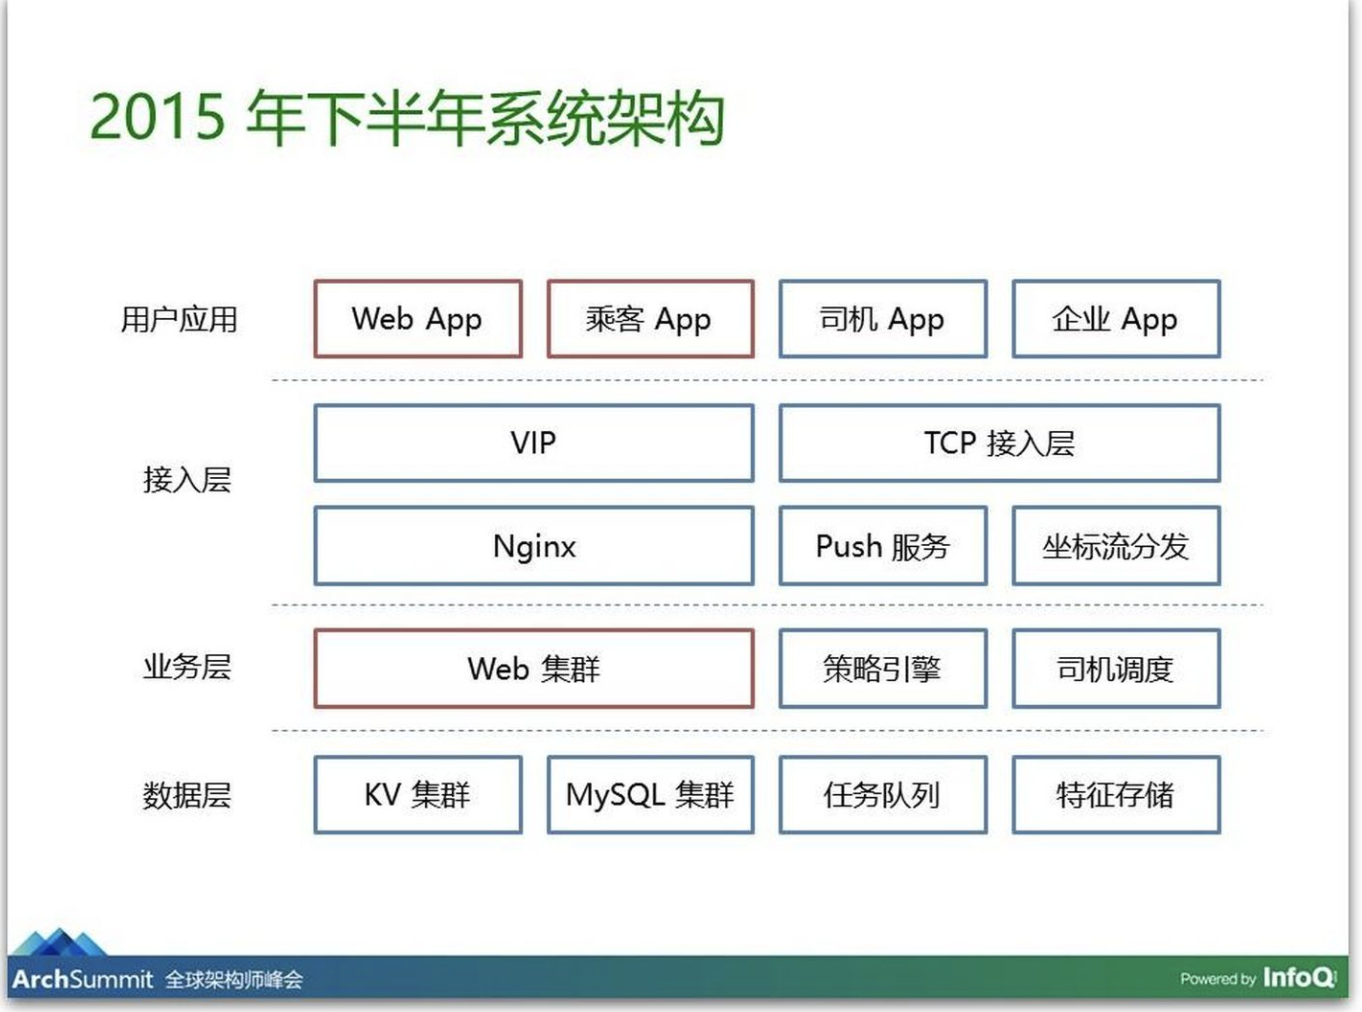
\includegraphics[width=1\textwidth]{fig/DIDI_Reconstruction_4.png}
\end{figure}

下面这张图可能会比较有趣。右边这个红色的球,代表的是重构之前App依赖的关系。当时我很想梳理一下App在模块之间是如何进行依赖的,然后我就写了一个脚本运行了一下,得到的结果让我很惊讶。我用蓝色的线表示正常的依赖,就是模块A依赖于模块B,A是B的上一层,B不会反过来依赖A,用红色的线表示异常的依赖,即A依赖B、B通过各种手段反过来依赖A,最后发现基本上都是红色的。做任何模块的拆分,发现不得不面临这样的问题:把任何一个模块取出来就等于把所有模块都取出来,实际上没有做拆分。所以,关键是需要解耦模块结果。这是iOS的情况,Android的情况更糟糕。

\begin{figure}[H]
    \centering
    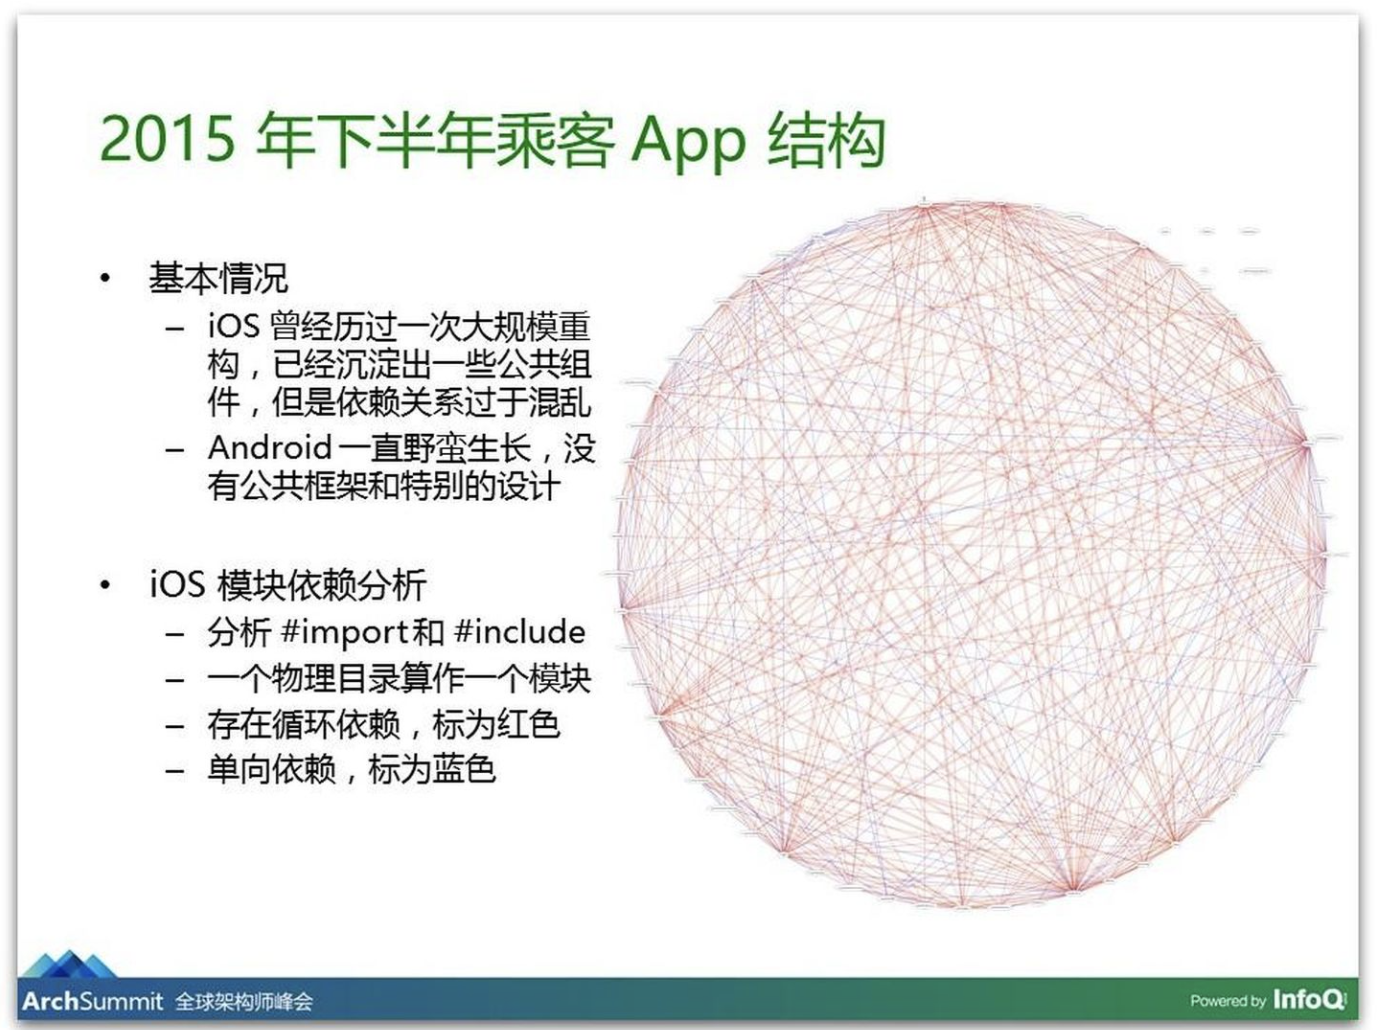
\includegraphics[width=1\textwidth]{fig/DIDI_Reconstruction_5.png}
\end{figure}

对于Web App来讲,最大的问题在于耦合性。以前滴滴只有出租车这个业务,最开始的Web App只有出租车,后来专车上线了,就在出租车里面加了专车入口,只是业务名不同界面会有小区别,后来加入了快车、代驾,都跟出租车差不多,没遇到太大问题。再后来有了顺风车,顺风车跟其他功能不一样,整体界面是预约型的,有乘客和车主两种模式。如果在老首页里面开发顺风车成本太大了,需要和出租车业务线的人一起开发业务模块,如果未来做迭代,这种开发模式将非常痛苦。老首页的模块也没有做拆分,代码散落各地,只是通过打包工具拼接在一起,没有做模块化,所以整体情况也比较糟糕。

\begin{figure}[H]
    \centering
    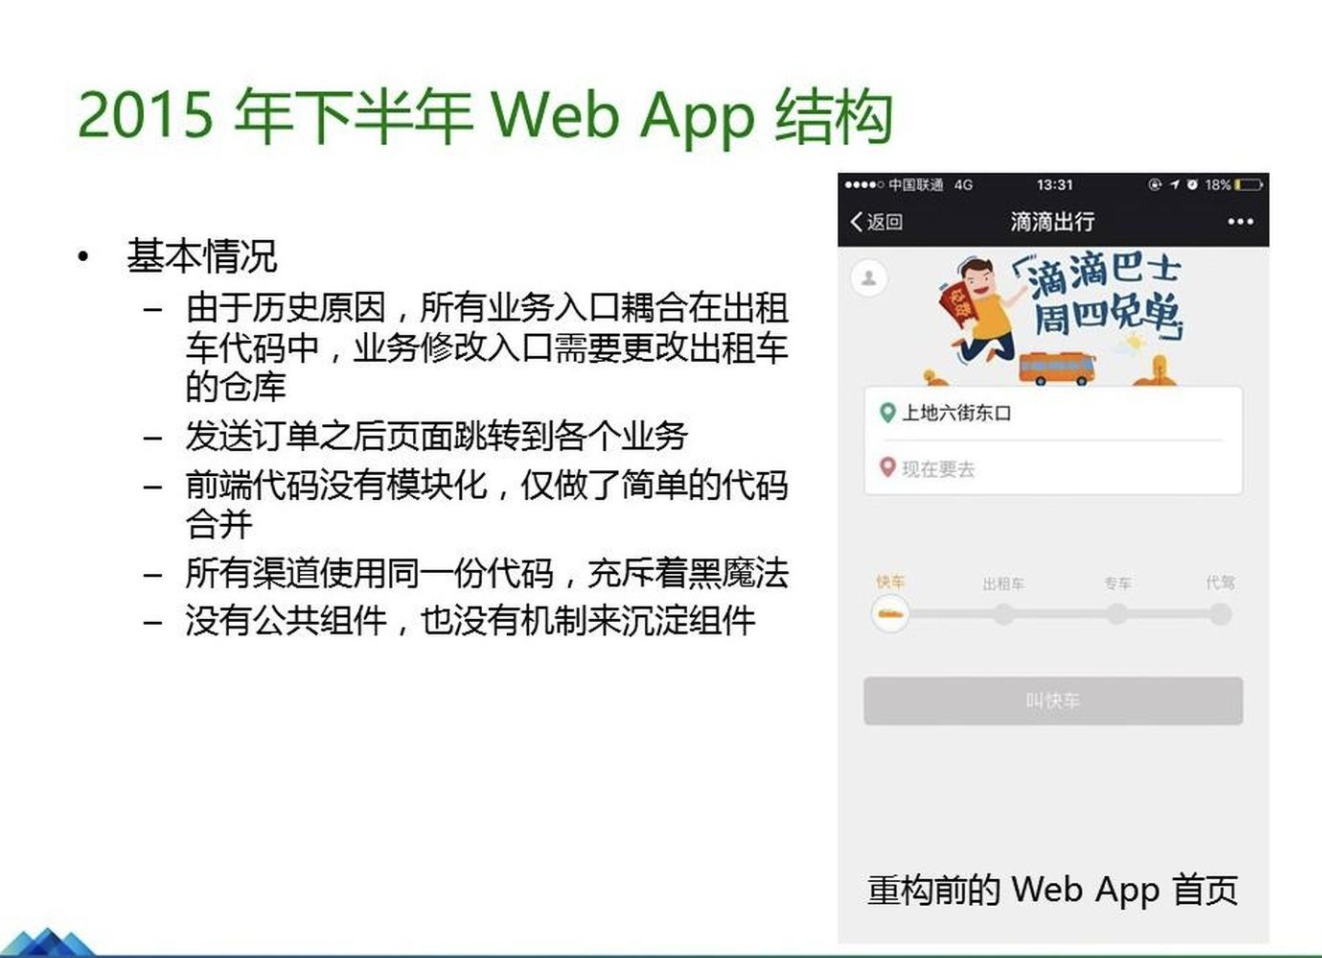
\includegraphics[width=1\textwidth]{fig/DIDI_Reconstruction_6.png}
\end{figure}

相比端,API稍好一点的是,API至少在业务维度上是分开的,出租车与专车、快车是分开的两个系统,放在两个仓库里面。不过API也有一个很大的问题,业务代码没有做服务化拆分,没有model 封装,业务所有的API和后台MIS都在一个仓库里,这对系统来说是非常大的一个隐患。

\begin{figure}[H]
    \centering
    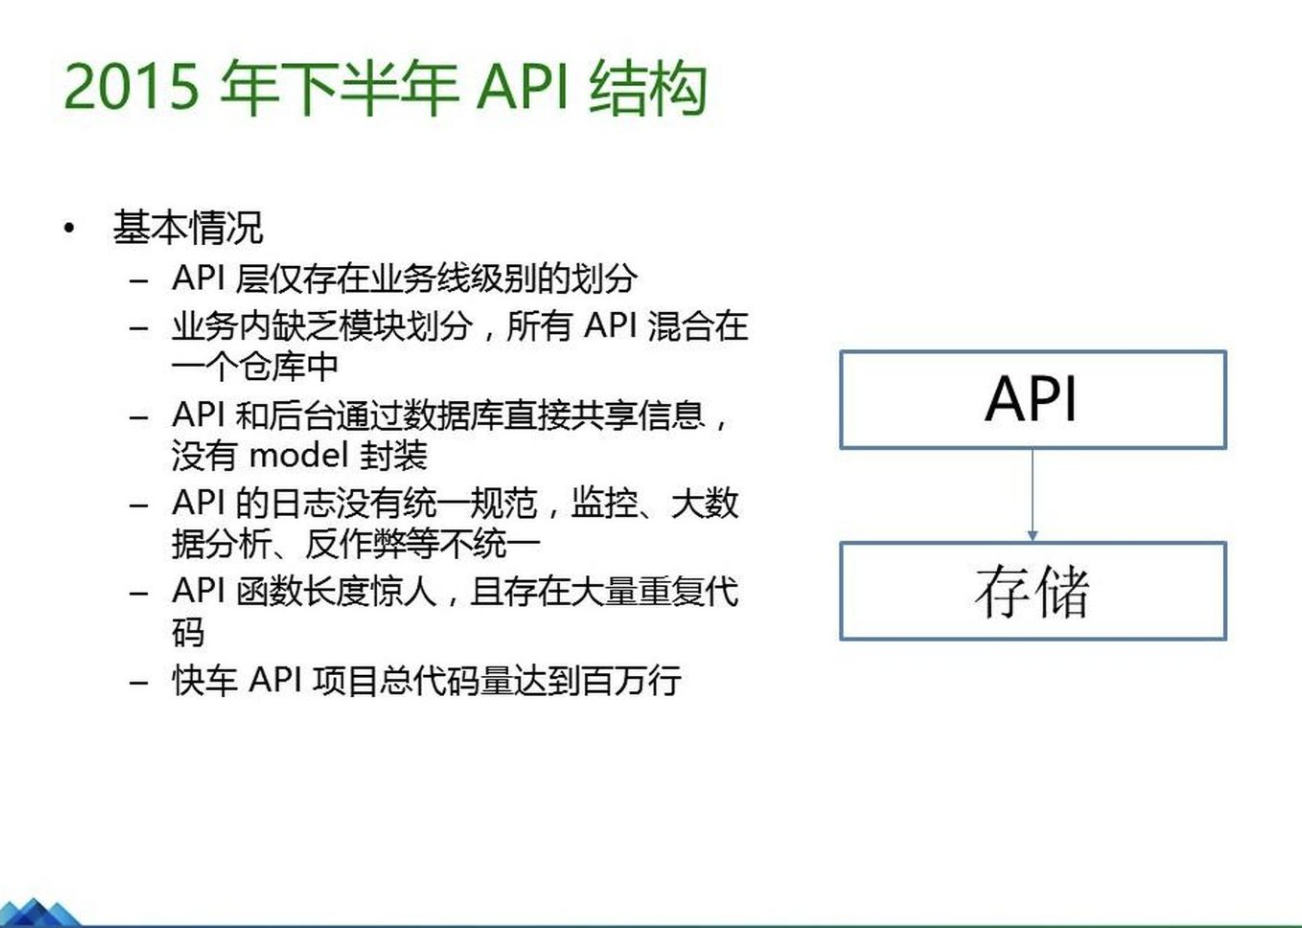
\includegraphics[width=1\textwidth]{fig/DIDI_Reconstruction_7.png}
\end{figure}

\section{该如何入手}
现状看上去很糟糕,要仔细思考才能入手。最基本的思路是把所有事情分类,就像整理自己家里一样,无论多乱,我们要做的事情就是将东西分门别类放好。因此,最关键的是要了解到底哪些东西应该放在一起,我们用颜色来比喻模块或者代码的归属,核心问题就变成这些模块到底是什么颜色。

\begin{figure}[H]
    \centering
    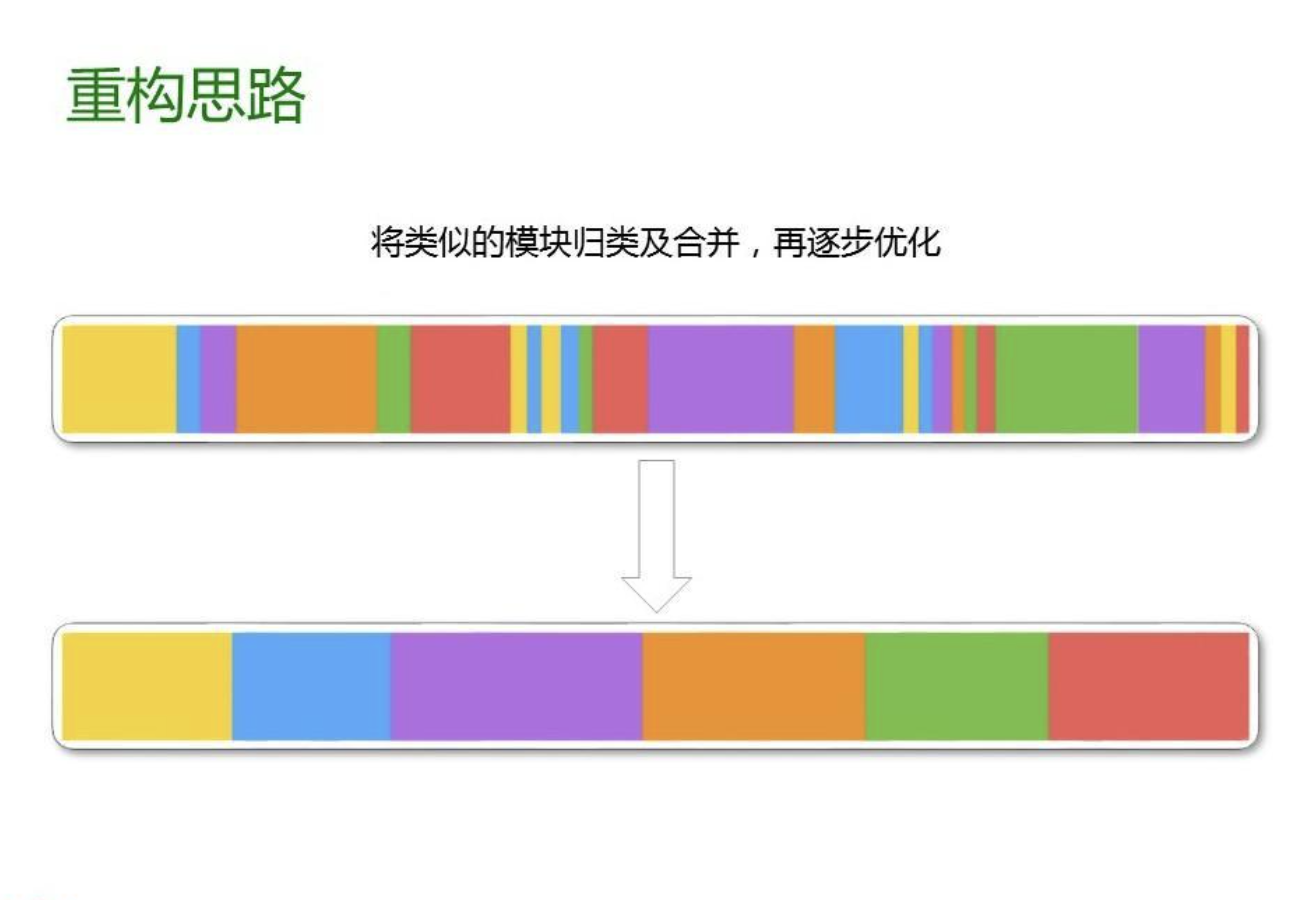
\includegraphics[width=1\textwidth]{fig/DIDI_Reconstruction_8.png}
\end{figure}

我们的思路是,先从前面,也就是从用户入口进行拆分,要先保证所有的模块是足够内聚的,由统一的团队负责。比如,出租车业务线可以完全控制自己的代码,能够写自己的客户端,也能够写自己的Web App,最终只是通过一些工程构建手段将多个业务整合起来变成一个完整的端。做到这一点之后,所有的业务迭代问题就迎刃而解了,因为业务间已经没有依赖和耦合了。这一步完成之后做的就是重新梳理业务,让业务根据自己模型特点进行一些重构。

最开始的时候,我们考虑的是怎么做代码治理和模块下沉。\textbf{代码治理本质上就是把各种模块进行染色、再把它们归类的过程}。代码治理最难的事情在于消除错综复杂的依赖。到底怎么做才对呢?首先,一定要把不同模块的代码放在不同仓库里面,使得模块能够物理上隔离。特别是Java、Obj-C这些静态编译的语言,一旦把代码仓库隔离就完全没有办法直接对其他模块产生依赖,至少绝对不会再出现循环依赖。再者,就看如何把循环依赖通过一些间接层隔离开,比如通过抽象接口隔离开,一点一点把代码拆到不同仓库。最后,有了这样一个简单的拆分之后,就需要考虑怎么让模块能独立的开发、测试、上线。独立的流程一旦独立起来,就意味着拆分基本上成功了。

\begin{figure}[H]
    \centering
    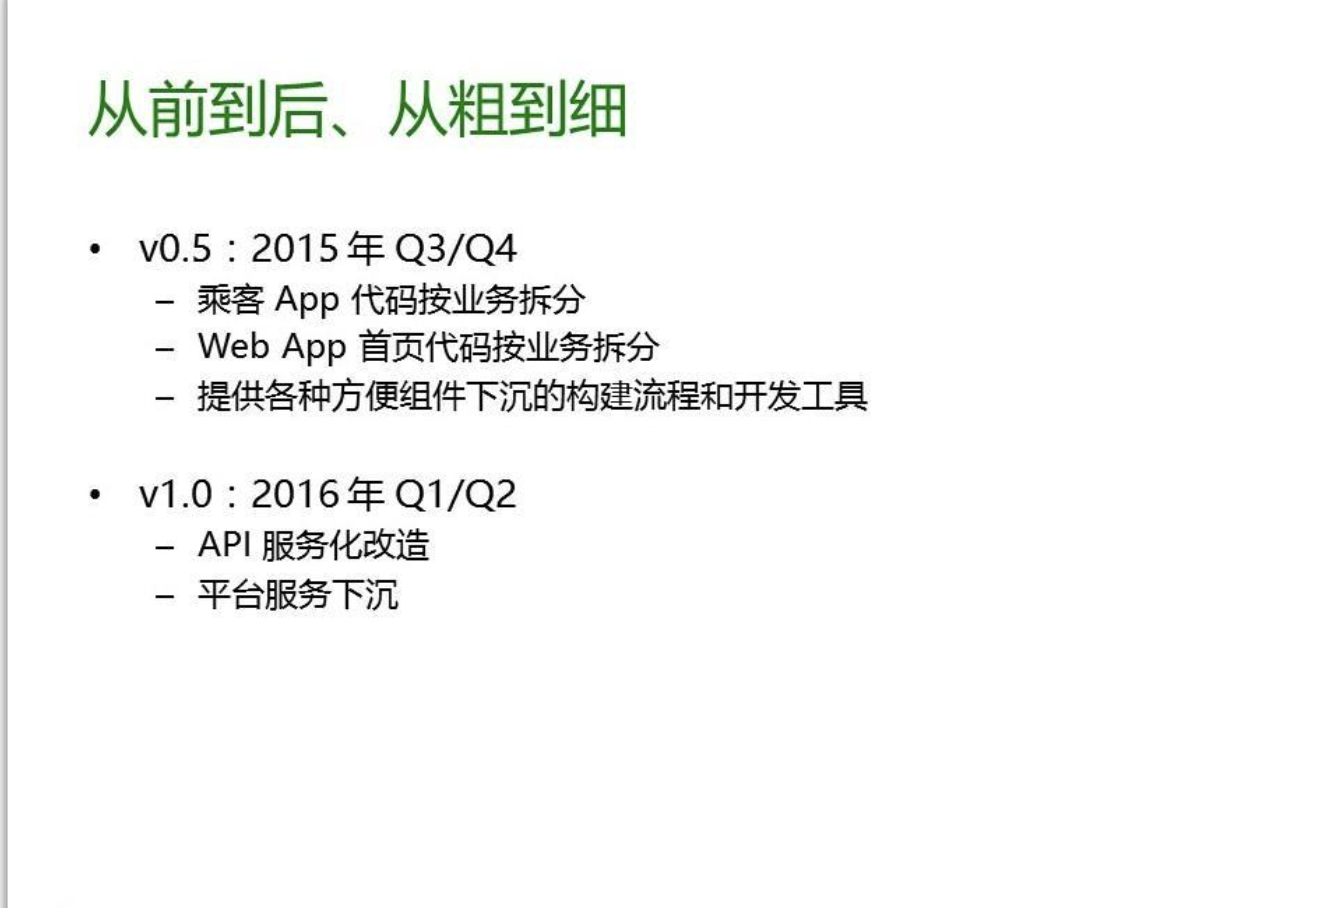
\includegraphics[width=1\textwidth]{fig/DIDI_Reconstruction_9.png}
\end{figure}

\textbf{模块下沉与代码治理息息相关}。如果只是要求把所有代码拆分,而没有合适的拆分方法,这件事情是无法推进下去的。对于程序员来说,他们内心总有一种冲动想做有意思的事情,比如封装一个很有意思的模块给更多程序员用。大家并非不想做封装,只是如果封装并共享出来的代价太大,就会影响大家的热情。

模块下沉是一种机制,一方面我们应该鼓励,另一方面还应该让大家发现这是一件不得不做的事情。如果仅仅对内公开模块列表让大家自由选择,达不到模块下沉的目的。因为人都很懒,不想思考太多,只想尽快把事情完成,大家往往倾向于复制粘贴,也不愿意额外花时间做下沉。怎么办呢?我们会给所有业务提供一个统一的SDK,里面包含所有能用的组件,大家必须使用它进行开发。如果业务模块稳定了并且比较通用,我们有工具和相应的简单机制把业务模块下沉下来,变成SDK的一部分,长期下去SDK会越来越大,只要SDK里做好分类和规划,上层就会越来越轻,我们可以真正专注于业务逻辑开发。

\begin{figure}[H]
    \centering
    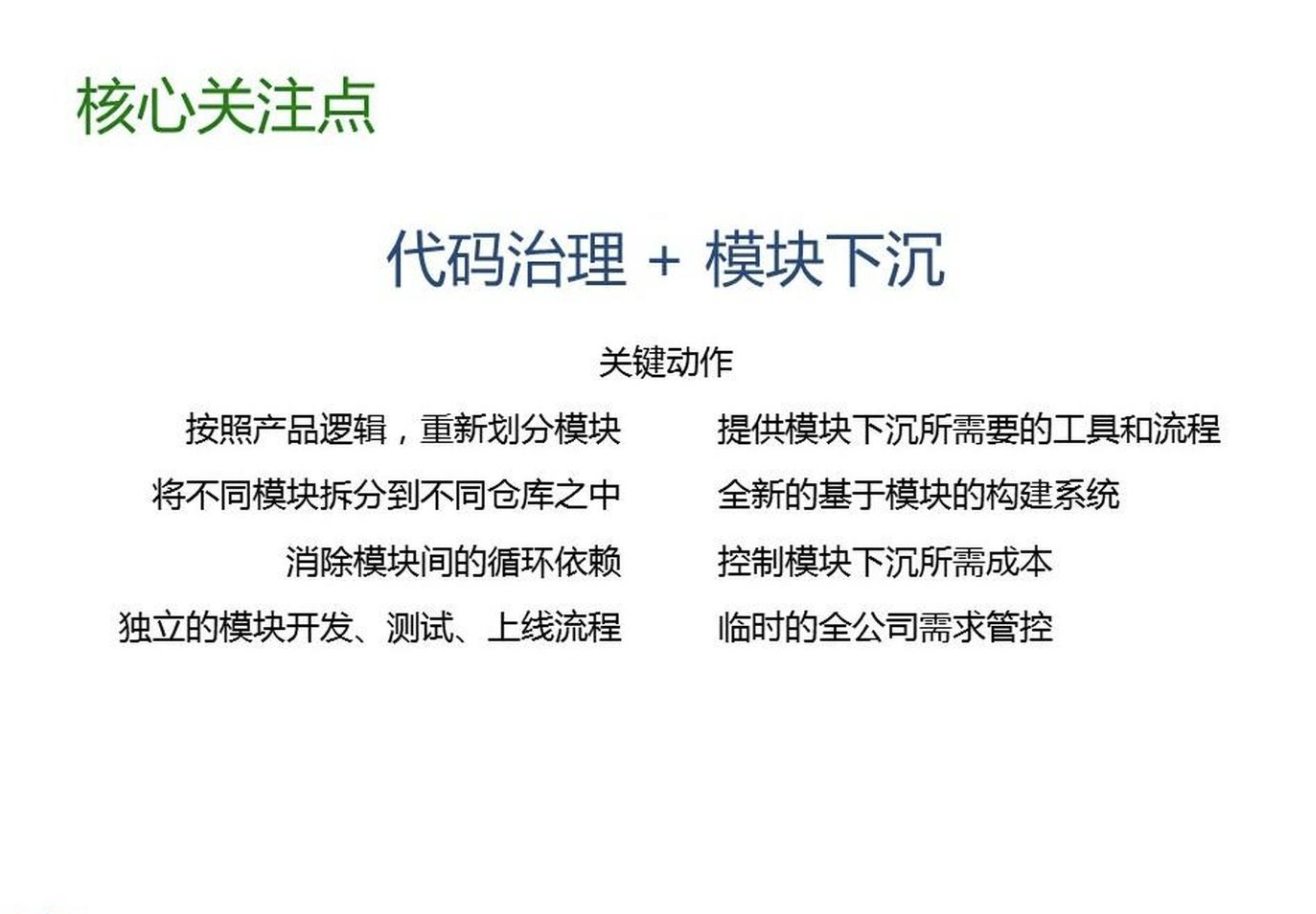
\includegraphics[width=1\textwidth]{fig/DIDI_Reconstruction_10.png}
\end{figure}

除了上面这些,最核心的一点在于,一定要把所有业务都做到“\textbf{无状态}”和“\textbf{异步化}”。

“无状态”这个概念在服务端比较容易理解。一般我们倾向于把各种业务做到无状态,这样容易做水平扩展。在客户端也是一个道理,也要考虑横向扩展性。一个简单的框架往往提供一些最基础的控件,比如按纽、列表,这些都不会耦合任何业务逻辑,所以很容易使用。但是当业务做起来,大家习惯将一些状态放到业务控件里面,这在一定程度上方便了,但是一旦需要将业务进行重构或者进行模块化下沉的时候,就造成了非常大的困难。例如,一个模块如果大量通过全局变量或单例跟上下游耦合,那么这个模块就很难复用和重构,这些全局变量或单例就是状态。所以,\textbf{我们在客户端也提出使用“无状态”的方式,把存储的信息都放到外面}。后面我会提到到底应该怎么样去做。

“异步化”也是解耦的方式。服务端的RPC类似于函数调用,如果参数变了,实现和调用的双方都要做改变,这很不透明,也不能够渐进式上线。我们用订阅/发布的模式对 RPC进行解耦,要求所有接口都要异步返回。在客户端也是这样,比如做数据的缓存,想优化网络,我们不能够期待这个函数是一个同步函数,一定用回调的方式接受所有参数。所以做设计的时候,只要是有可能发生网络请求或者访问磁盘,在客户端也尽量异步请求数据。

刚刚讲的都是相对比较抽象的内容,接下来会说一下滴滴的业务形态本身。

滴滴是一个出行的平台,涵盖的是整个出行领域所有的出行需求。大家出行到底想要什么?就是到达自己想去的地方。实际上,我们的模型可以做得非常抽象和简单。比如,我想要打快车去机场,我就是一个需求方,我的需求会发到很多服务者那里去,服务者会根据特征进行一些匹配。最基本的特征是服务能力,如果服务者能够开快车并通过了能力验证,这个需求就有可能发给他。如果开出租车的也有能力开快车,但是他还没有在平台上验证这个能力,就只能开出租车。一个人可以验证很多服务,白天可以开快车,晚上可以做代驾,做不同的事。

\begin{figure}[H]
    \centering
    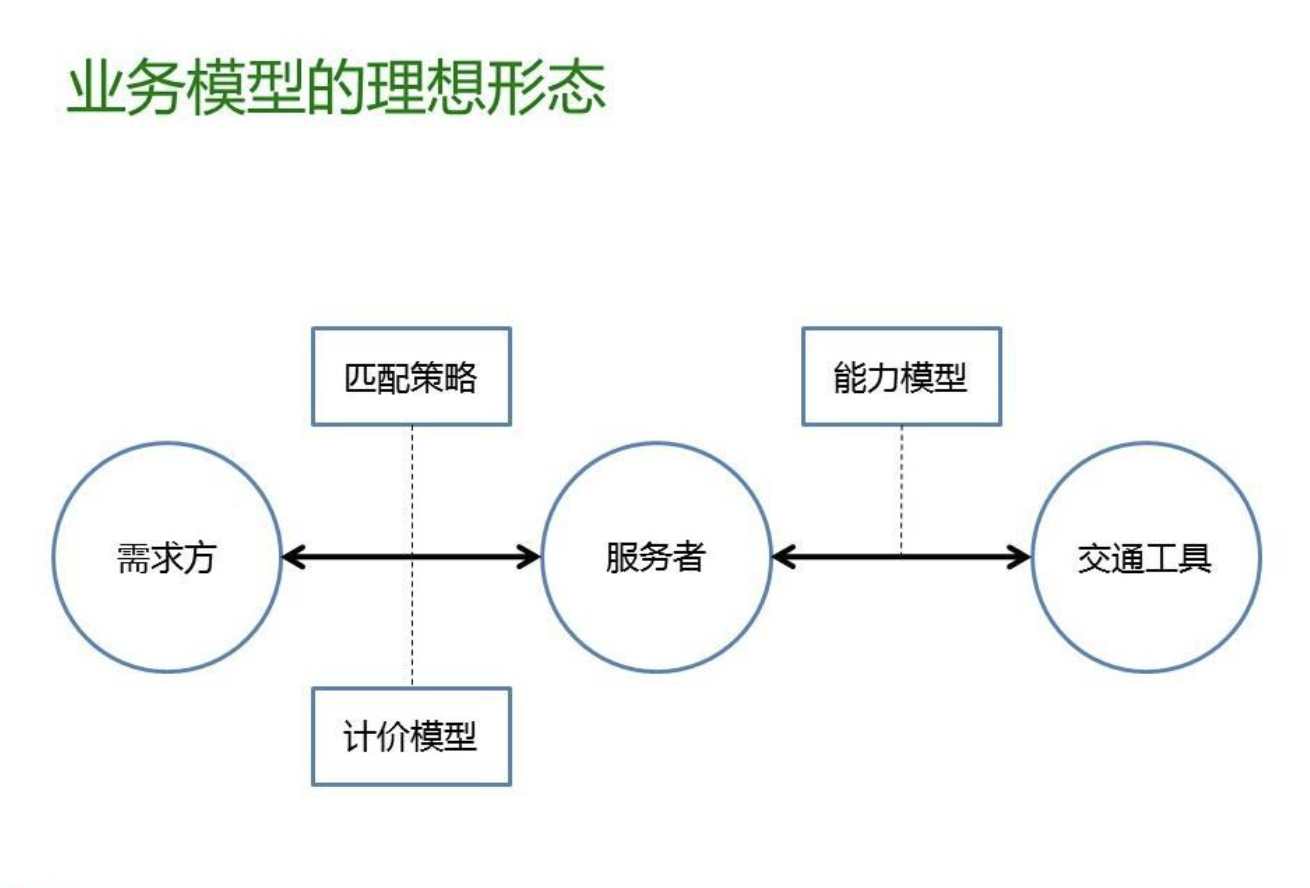
\includegraphics[width=1\textwidth]{fig/DIDI_Reconstruction_11.png}
\end{figure}

服务和需求的匹配是通过\textbf{计价模型和匹配策略}来实现的。发送需求的时候需要选择计价模型和车的类型。快车和专车服务过程大同小异,但是价格差别很明显,专车价格会贵很多。通过匹配策略可以实现各种需求的匹配。例如,选择了拼车,这个需求会尽量匹配已经有拼友和顺路的车。如果选择专车,可以要求这辆车在指定时间来接人,这时候匹配策略会优化倾向这种方式。

滴滴所有的业务基本上都是以这种模式运转的,所有功能都是核心主干或者旁路,只要把业务模型抽象出来,基本上就能够满足大部分的业务了。

基于这样的想法,我们就思考如何设计真正高度抽象的工具。简单起见,我们把滴滴出行的过程抽象成一个框架(见下图),这并不是完整的框架。有颜色的地方表示出租车、快车、专车、代驾共同的流程,只要组合各种流程就可以实现整个业务形态的能力。在这个框架里可以定制所有业务形态的车标、提示语、匹配的模型、计价模型等功能。当时梳理这个抽象的时候,我们感觉非常兴奋,因为这意味着在这个基础之上就可以简易扩展出滴滴未来的业务形态。只要滴滴还是在做需求和服务的匹配,基本上就离不开这样一种套路。

\begin{figure}[H]
    \centering
    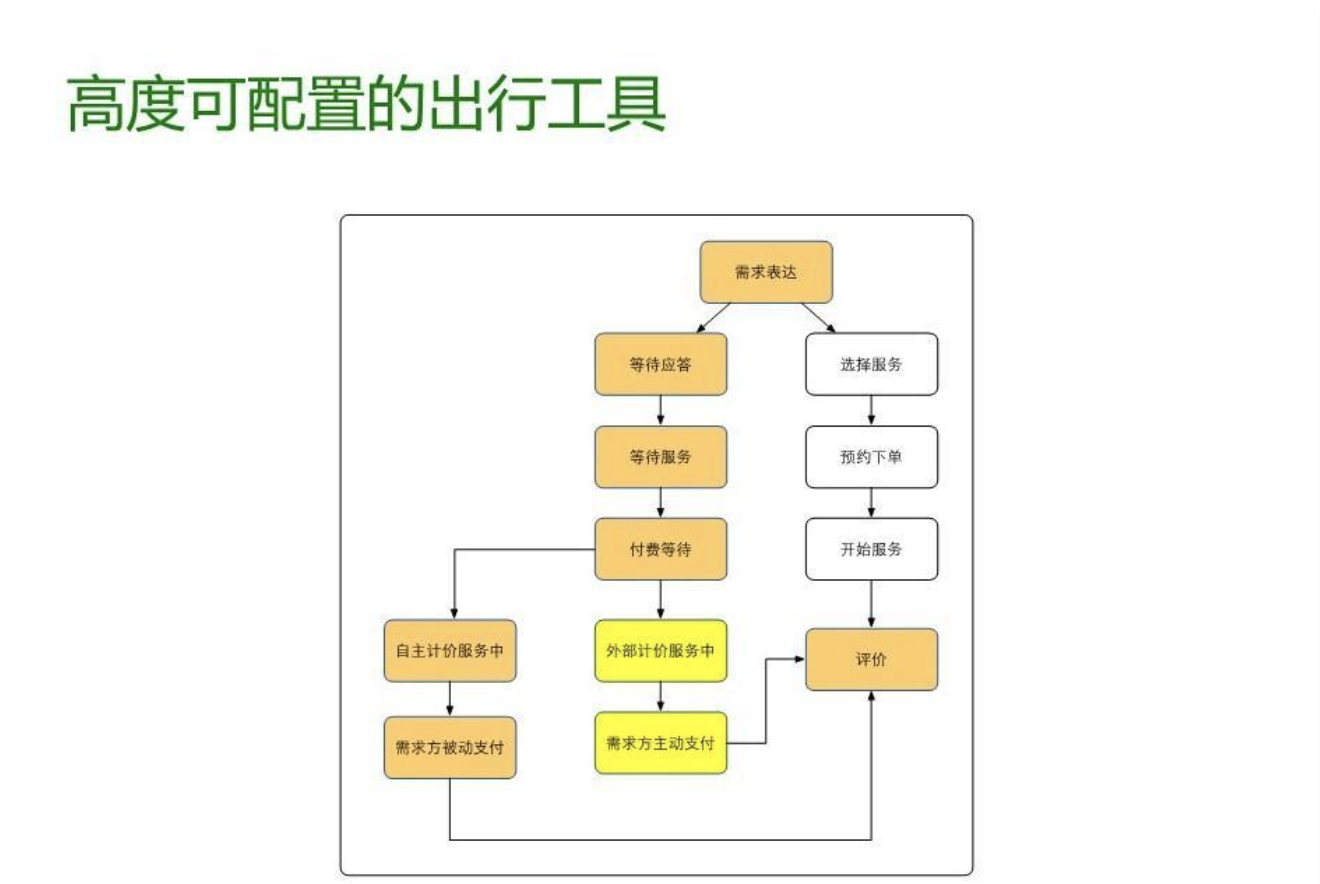
\includegraphics[width=1\textwidth]{fig/DIDI_Reconstruction_12.png}
\end{figure}

\section{客户端怎么拆}
然后我们开始落实到具体该怎么拆的问题。

首先就是客户端,最重要的是需要将业务拆出来。以前所有业务放在同一个仓库里,如果不小心提交了一段错误代码就会带来灾难性的后果,所有业务工作可能都会受到影响。以前编译速度也很糟糕,大家可以想象,每次下载代码都会有几个头文件发生改变,由于循环依赖的缘故几乎所有文件都要重编,二三十分钟后才能重新调试,这个过程让人极度崩溃。对于iOS,我们用cocoapods把业务拆到不同的pod里面;对于Android,我们把业务拆分打包并用Maven管理起来。

我们拆分方法如下图所示,其中虚线框部分展示的是公共框架,最开始没有很细致分割,只是把它放在一个独立仓库里,保证依赖关系充分清楚,后面就可以随时把代码独立出来,使其变成单独的模块。

\begin{figure}[H]
    \centering
    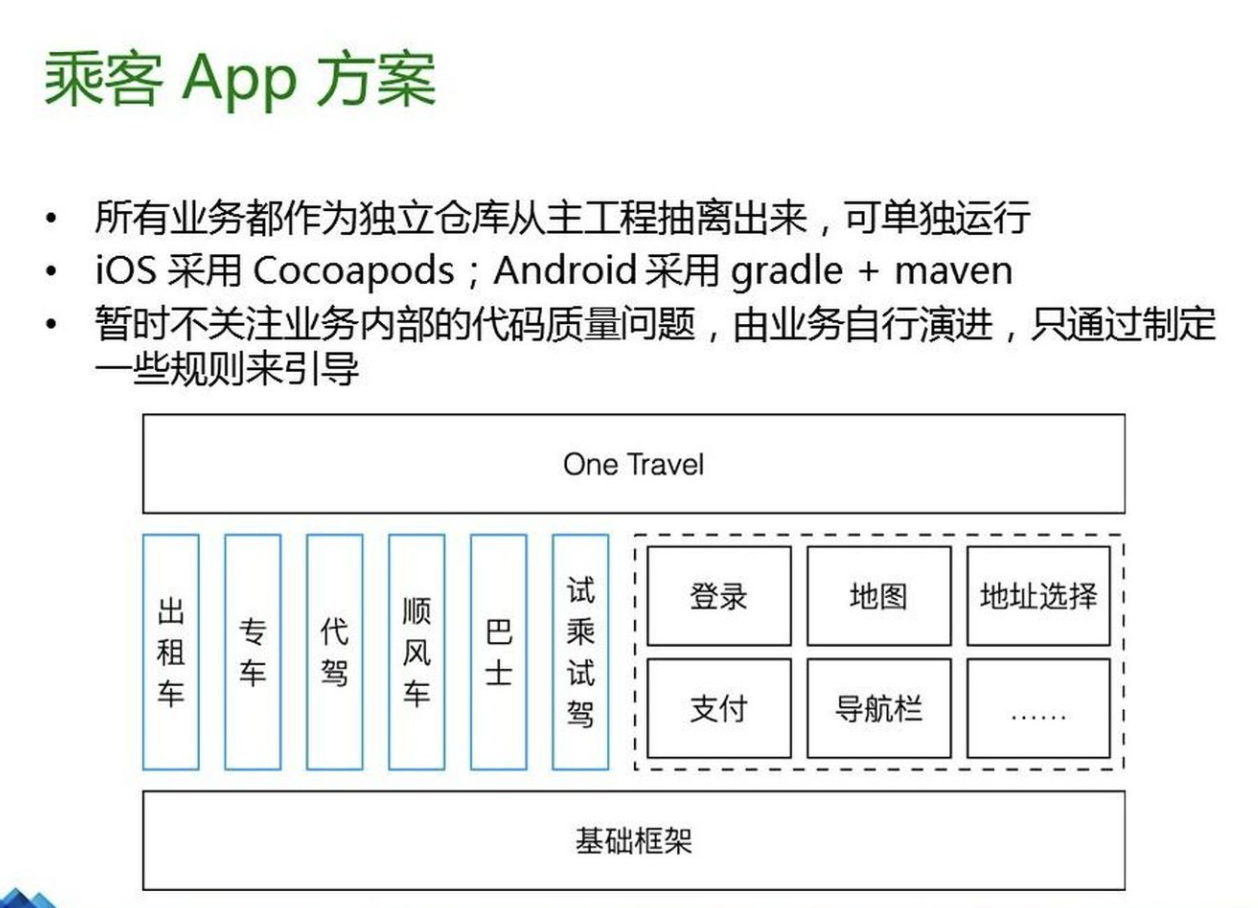
\includegraphics[width=1\textwidth]{fig/DIDI_Reconstruction_13.png}
\end{figure}

同时,我们也在开发构建系统。原生的构建系统使用起来会有很多问题,它并不支持多人并行开发,如果要实现一个舒适的工作流就需要定制。我们还做了网络和日志的封装,将其放在下层。还有一个业务整合的基础框架,包括滴滴出行的App界面框架、首页导航栏,各种业务可以注册自己的入口,并在导航栏里进行切换。业务之间没有任何代码耦合,比如出租车和专车业务没有关联性,那么代码也没有任何相关的地方,这意味着开发出租车业务的时候,完全没有必要实时更新专车代码,集成的时候也不会因为专车代码而造成问题。最顶层的One Travel可以通过简单的配置分业务包,比如可以输出只有出租车业务的包,在这上面开发测试速度比较快,整体也会比较灵活。One Travel里面只有极少的代码,未来会改成没有代码、通过脚本就可以生成的项目。

怎么做页面的解耦?下图中是一种\textbf{类似数据库缓存的设计}。从客户端角度来看,如果把服务器当做一个数据库,最终状态存储在服务器,而客户端里存着的是跟服务器同步过的最新状态的缓存。客户端不太可能做到精确的数据同步,一定是每隔一段时间同步一次,或者是在关键节点上靠服务器推送得到订单状态变化。

客户端的业务代码其实不关心究竟是如何同步状态的,所以我们专门写了一个缓存服务器状态的Store层,它是热数据。如果不需要最新状态的数据,业务读取Store时可以读到上次同步的数据,假设此时Store从未同步过状态就会自动读取最新状态;如果业务一定要最新状态的数据,那么就显示要求缓存失效,这样Store就会再读取一次获取最新的信息。Store还可以自动设置失效时间长度,这个机制跟跟做数据库缓存是一样的,为了性能的平衡,要保证读出准确的数据,同时性能也要最优。同时,Store也有责任负责数据更新,当客户端变化可能会让服务器状态变化时,Store可以自动让相关状态失效,这也是管理缓存的一般做法。

\begin{figure}[H]
    \centering
    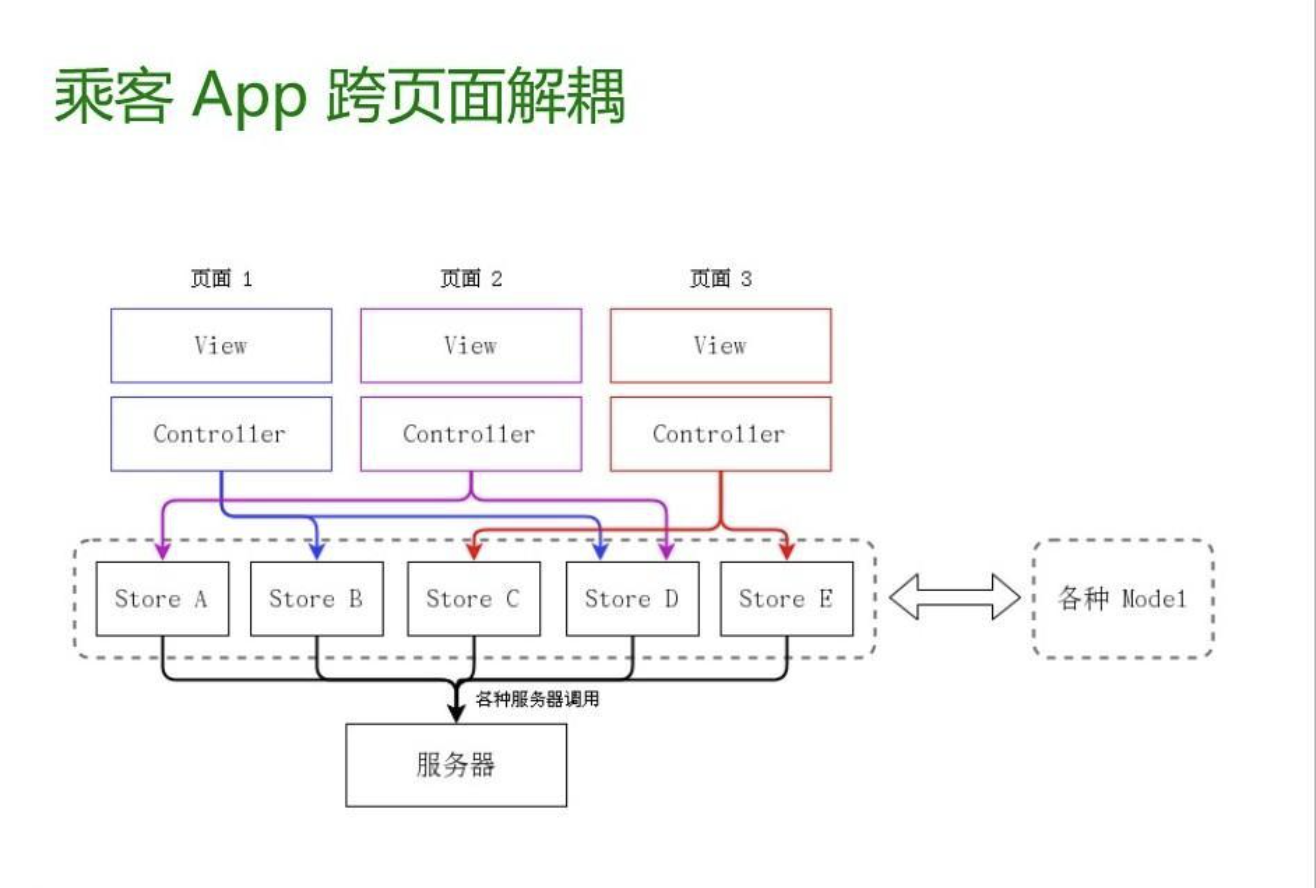
\includegraphics[width=1\textwidth]{fig/DIDI_Reconstruction_14.png}
\end{figure}

做了这样一些解耦之后,令人惊喜的是,我们发现所有界面是可以随意跳转的,虽然没有从发单直接跳到评价的必要性,但实际上只要有这个架构,就可以从界面A跳到界面B,不会有任何问题。如果跳到另外一个界面,没有发现必要的数据,就从服务器读取,它自己也会报错,整个逻辑非常清晰。如果需要在流程A和流程B之间再增加一个流程C,我们可以把流程C直接加进去,流程C没有破坏A和B之间的依赖,因为原本A和B之间也没有什么依赖。

我们也做一些App的组件化,把从服务端API到客户端逻辑打包在一起,引用客户端组件就可以实现完整功能。实际封装方法略微有点复杂(编者注:可以阅读另外一篇文章《滴滴的组件化实践与优化》)。图中所示是做平滑移动组件,地图上有很多车在移动,这些车就是地图上的额外信息,把这些车挂在地图上。如果这个控件不存在,地图上就没有车,控件存在,地图上就有车,只要在上面启动控件就好了。

\begin{figure}[H]
    \centering
    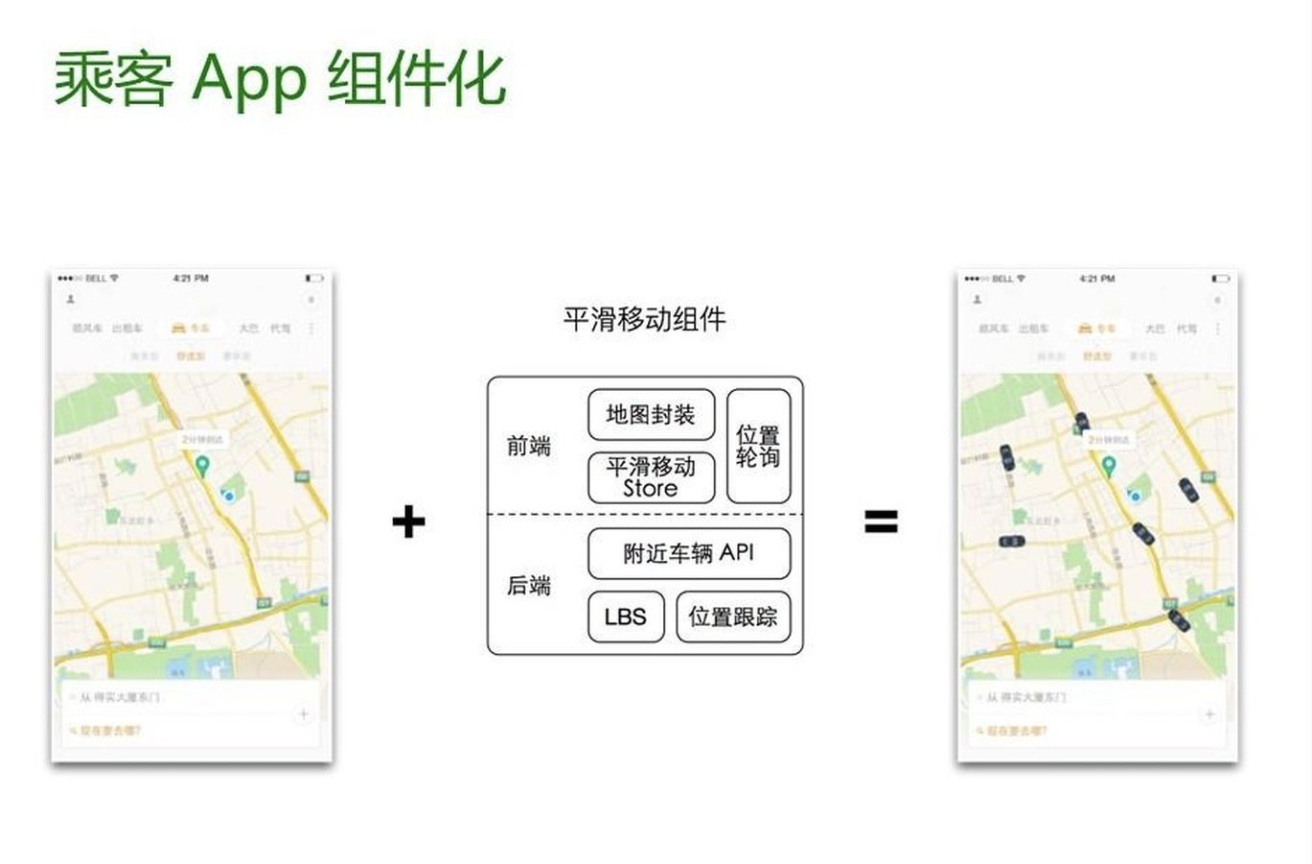
\includegraphics[width=1\textwidth]{fig/DIDI_Reconstruction_15.png}
\end{figure}

App集成也采用了异步和无障碍的做法,每个业务只需要在仓库里面测试完之后直接打tag,之后就能自动生成整个所有业务的ipa/apk包。

\section{Web App怎么拆}
接下来讲Web App的拆解,这实际上是纯工程的解耦。首先,我们需要实现一个简单的公共框架,这跟业务是无关的。我们使用scrat和webpack来实现工程化,将首页拆分成了许多组件,所有的业务可以根据不同配置选择使用哪些组件,同时也保证页面风格的统一、功能的稳定。如果网络比较糟糕,我们会做一系列的降级,首先出来的会是一些统一的控件,比如上车地点、目的地、广告等,之后会根据定位的结果得到当前开通的业务线列表,并加载业务代码,然后默认选择当前业务线的逻辑。如果业务线代码加载好了就开始渲染,如果业务加载出错或代码执行出错,业务就会被隐藏。业务线之间也是完全解耦的,大家可以通过公共框架提供的事件机制来通信,但不允许业务之间直接通信。线上的Web App就是如上图所看到的,每个业务线都有一段独立js代码,第一次加载相对较慢,会看到很多请求,如果业务线代码没有更新,下次打开就完全不走网络请求。

\begin{figure}[H]
    \centering
    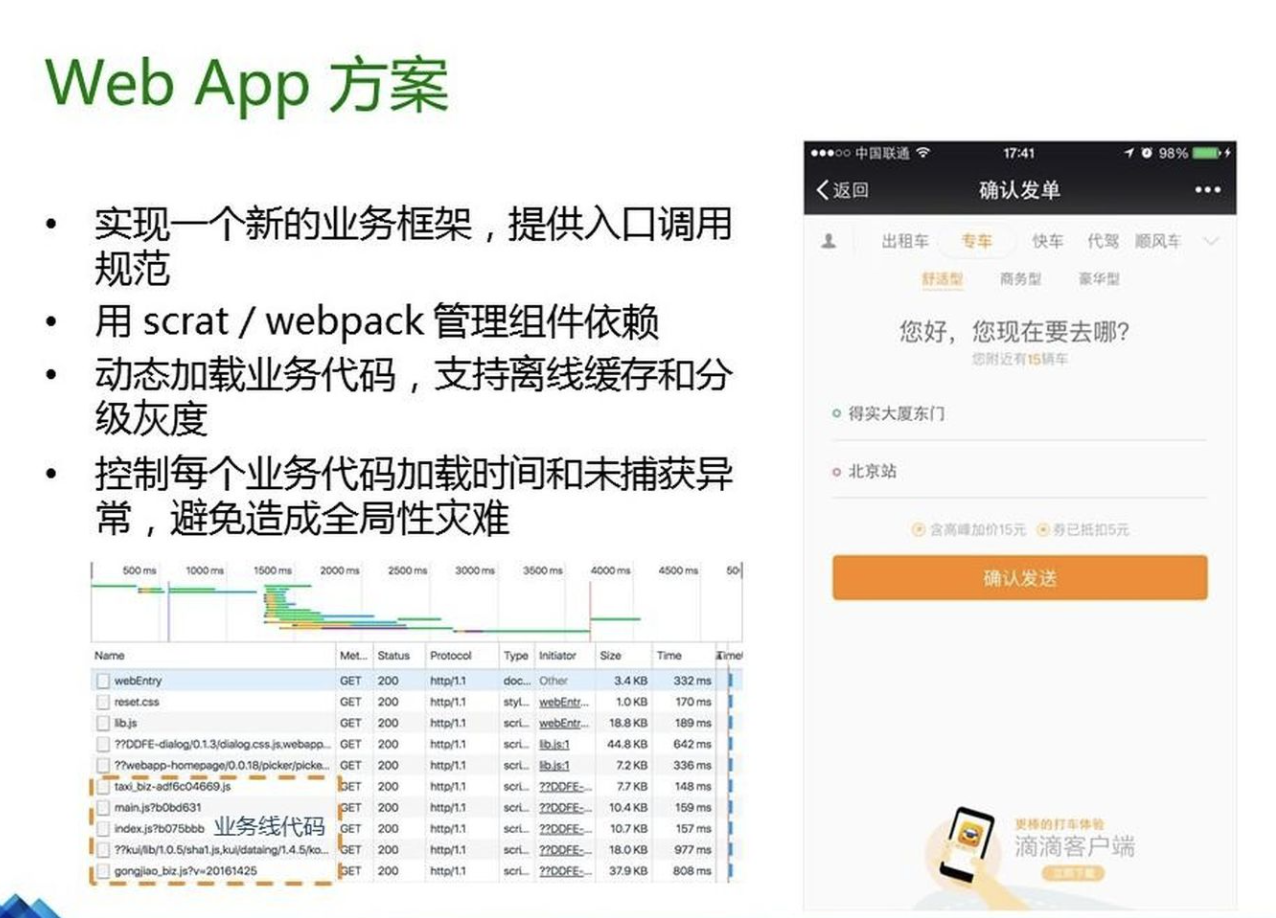
\includegraphics[width=1\textwidth]{fig/DIDI_Reconstruction_16.png}
\end{figure}

我们也做了很多控件,这是内网发布的一些控件(见下图),每个业务只要关注自己的业务逻辑即可,公共的功能都可以使用控件。特别是选择地址的控件,它把前端界面交互和后端API都打包在一起,和客户端一样,只要引用它,就可以直接在Web App使用,无需任何服务端的开发。

\begin{figure}[H]
    \centering
    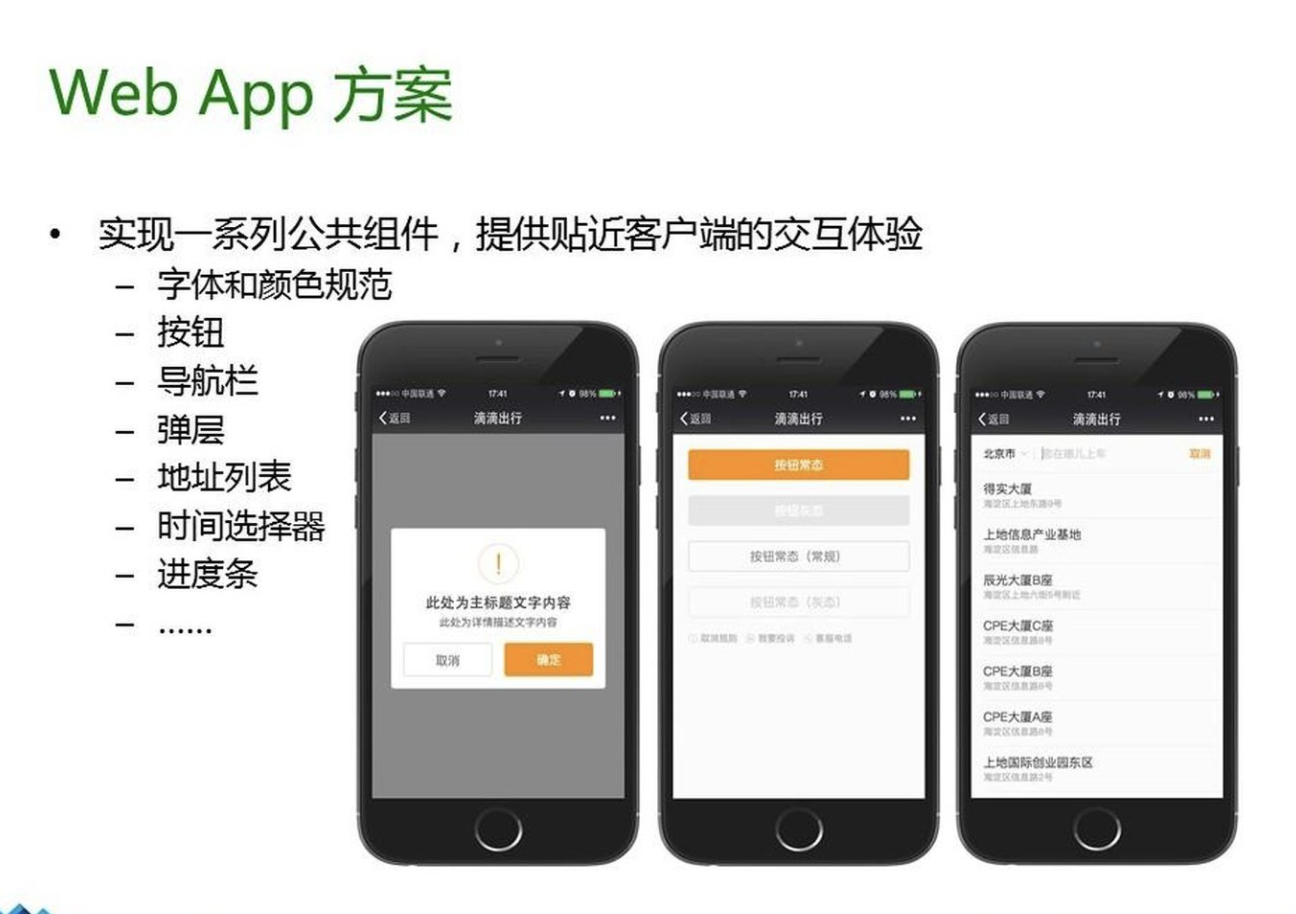
\includegraphics[width=1\textwidth]{fig/DIDI_Reconstruction_17.png}
\end{figure}

\section{服务器API怎么拆}
关于服务器API的拆分,我们最开始希望一次性实现理想方案,但是这个理想方案遇到一些问题。

我先来谈谈理想方案是什么。首先,\textbf{滴滴业务一般都是基于订单流转推动各种业务动作}。为什么会发生订单流转?是因为对乘客和司机做了一些操作,如果想象成一个客户端系统,就有点类似于触发各种用户事件。客户端动作根本上决定了信息该如何流转,所有事情都应该在客户端触发,触发之后来到了组件这一层,所有动作进行消费,然后进行下一步操作。比如,用户提出一个需求,发单对需求进行过滤,判断是哪种需求,然后进行一些检查。快车有拼车和不拼车两种,发单的时候就可以知道是拼车还是不拼车,对于统一订单系统来说这就是个标志。无论拼不拼,这个单对用户都一样,无非就是消耗多少人民币、消耗几个座位还是消耗整辆车的问题。之后分单系统会进行订单的匹配。一旦匹配成功,客户端有很多动作,司机确认接单,乘客可以看到确认。如果直接做成消息,客户端和服务端用一条总线连接,问题就解决了。

\begin{figure}[H]
    \centering
    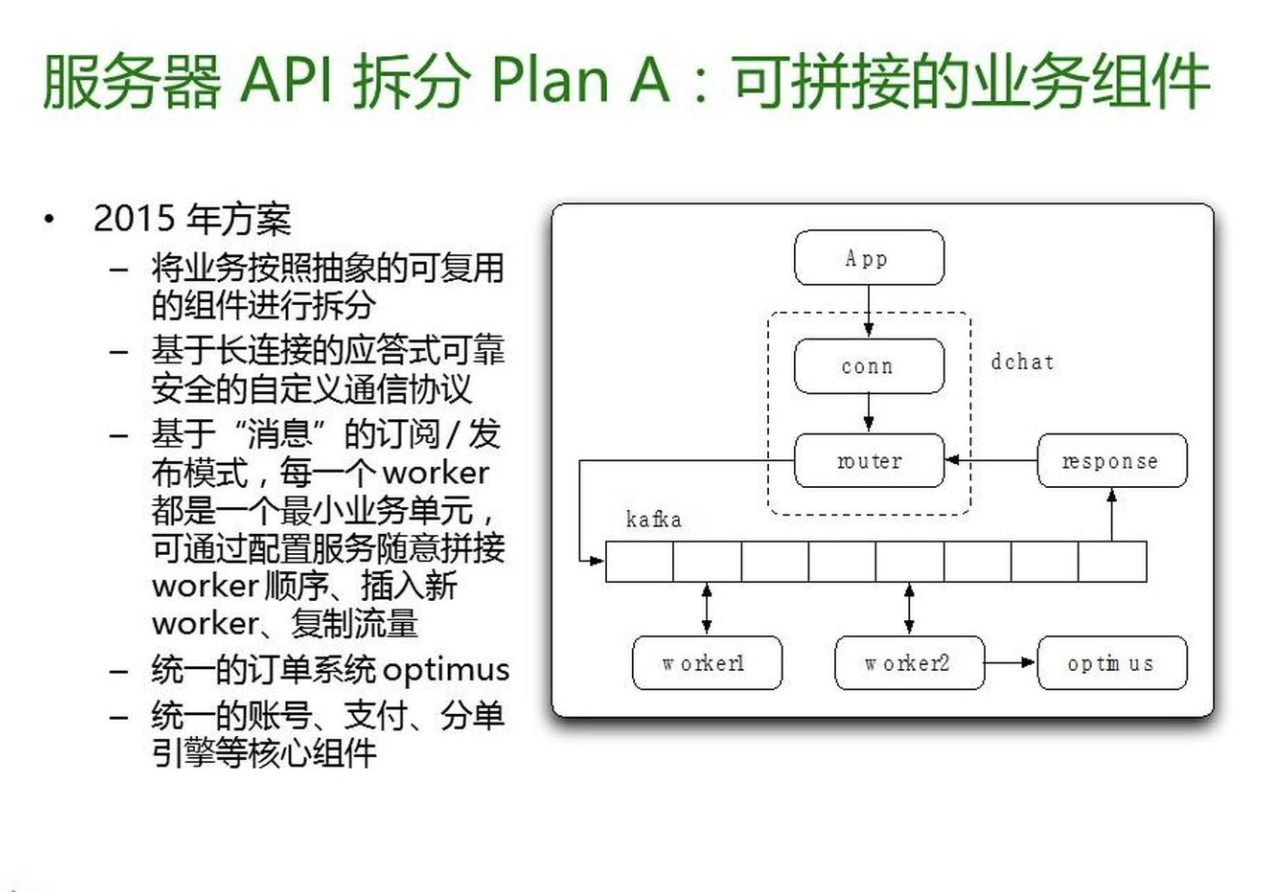
\includegraphics[width=1\textwidth]{fig/DIDI_Reconstruction_18.png}
\end{figure}

这里有一个很大的优点——可拼接,所有东西都组件化了。但是最大的问题在于抽象程度非常高。这是函数式的思想,要求所有的Worker都是纯函数,纯函数是非常高的要求,上下文状态必须要通过参数才行。我们发现很难做到这一点,因为所有系统必须有状态,一旦这样这个纯函数就不是纯函数了,要依赖外部的变量。与面向对象设计的思路差异非常大,做函数式设计时很容易陷入一些抉择当中,如何定义输入、输出,如何划分流程。有一些流程划分成三段式,中间的流程异步调出去,又异步调回来继续后续流程,这种设计让人很纠结。函数很依赖异步化,异步化会让数据流变得复杂。我们思考数据流的流向,以及每次数据流在流转的时候都需要设置的输入、输出。最终,这个方案并没有实施,虽然我们开发了接近半年的时间。

\begin{figure}[H]
    \centering
    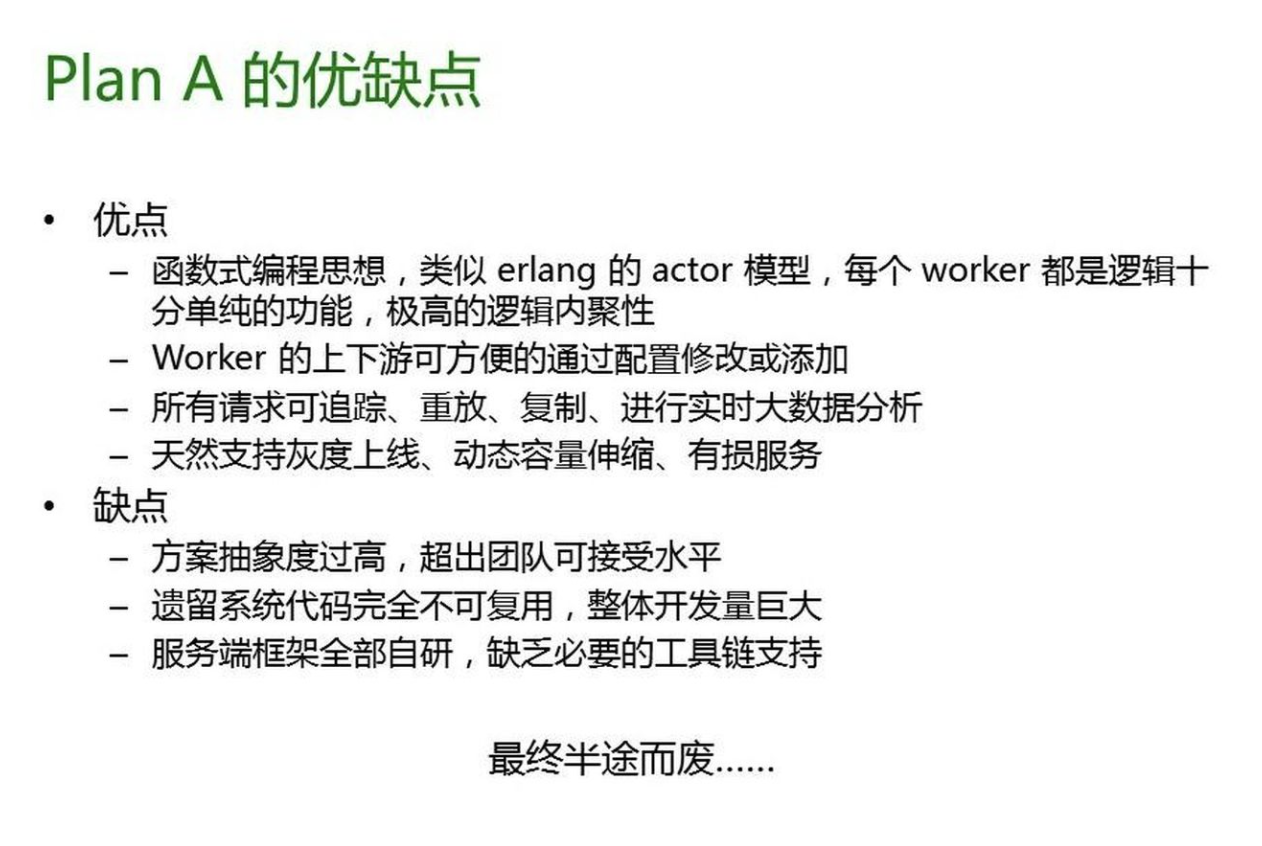
\includegraphics[width=1\textwidth]{fig/DIDI_Reconstruction_19.png}
\end{figure}

2016年,我们又重新思考了这个问题,这次是比较简单和现实的方法。首先我们进行了一些代码的隔离,把代码分开,之后对系统按照刚才讲的模块进行面向对象的抽象,比如发单就是单独的系统,订单也是一个单独的系统,支付的收银体系是一个系统,评价体系是一个系统。每一个系统变得很简单,互相之间用RPC调用关联起来。

\begin{figure}[H]
    \centering
    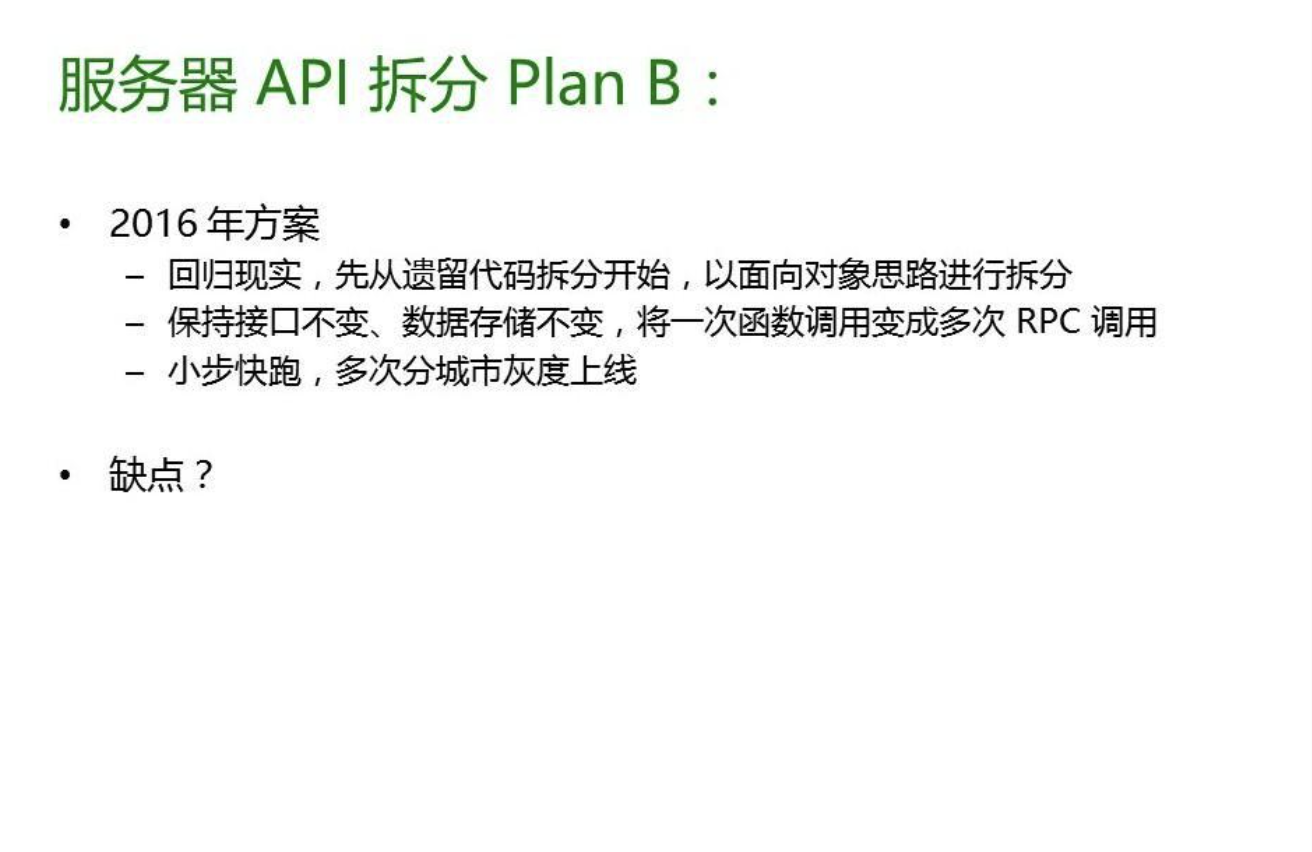
\includegraphics[width=1\textwidth]{fig/DIDI_Reconstruction_20.png}
\end{figure}

这会有什么缺点呢?长期来讲缺点还是比较明显的,就是不容易扩展。现在我们设计的模型是来源于当前业务现状,如果业务发生改变,比如多了一种车型,就会遇到该如何扩展的抉择:应该提供更多API接口满足新的业务功能,还是在原有API修改上提供更多参数。两种方法看起来都可以,但是本质上我认为无论用哪种方案都会使模块本身变得越来越臃肿,其实都是把很多种东西融合在一起,并不是很理想。当一个服务臃肿到一定程度之后又会出现以前的问题,又要再次做拆分和重构,甚至整个RPC调用流程都会发生很大震动。

从项目整体实施效果上来讲,这次重构最主要是解决了开发迭代的问题,能够让迭代速度更快。让我们比较意外的情况是,重构前客户端crash率非常高,重构中我们对代码进行了非常多的修改,同时还在用户体验上做了很多优化,但最终crash率反而大幅下降,从以前1\%降低到0.3\%。重构后各个业务团队的开发模式发生了根本的变化,以前是各个业务各耦合在一起进行开发,现在各个业务都能独立开发,互不干扰,同时平台还会不断产出更多的公共组件。

\section{如何避免重蹈覆辙}
最后提一下如何重蹈覆辙。我认为,所有的设计应该是自上而下,先从产品层面上规划核心业务的模式,然后考虑如何让产品技术实现它。如果把业务模式描述成如图所示的核心循环,会非常清楚。我们不仅要考虑现在,还要考虑未来。如果让整个架构保持健康,就要考虑什么功能是真正紧密相关的。比如在服务端,直觉上感觉各种不同的发单应该是在一起的,但实际上并不是这样。不同车型的发单接口互相之间并没有什么联系,每一种发单都会有独特的个性化定制,这些定制才是真正应该跟发单紧耦合的东西。所以我们应该从产品角度上考虑,把一种发单所调用的所有相关API放在一起,服务端发生变化,调用的组件也会发生变化,做到发单闭环。刚刚提到的今年服务端的重构的方法,实际上并没有让各个子系统打通,这是一件很遗憾的事。未来如果开发一些新需求,肯定还会涉及多个模块、团队,避免不了一些沟通成本。

\begin{figure}[H]
    \centering
    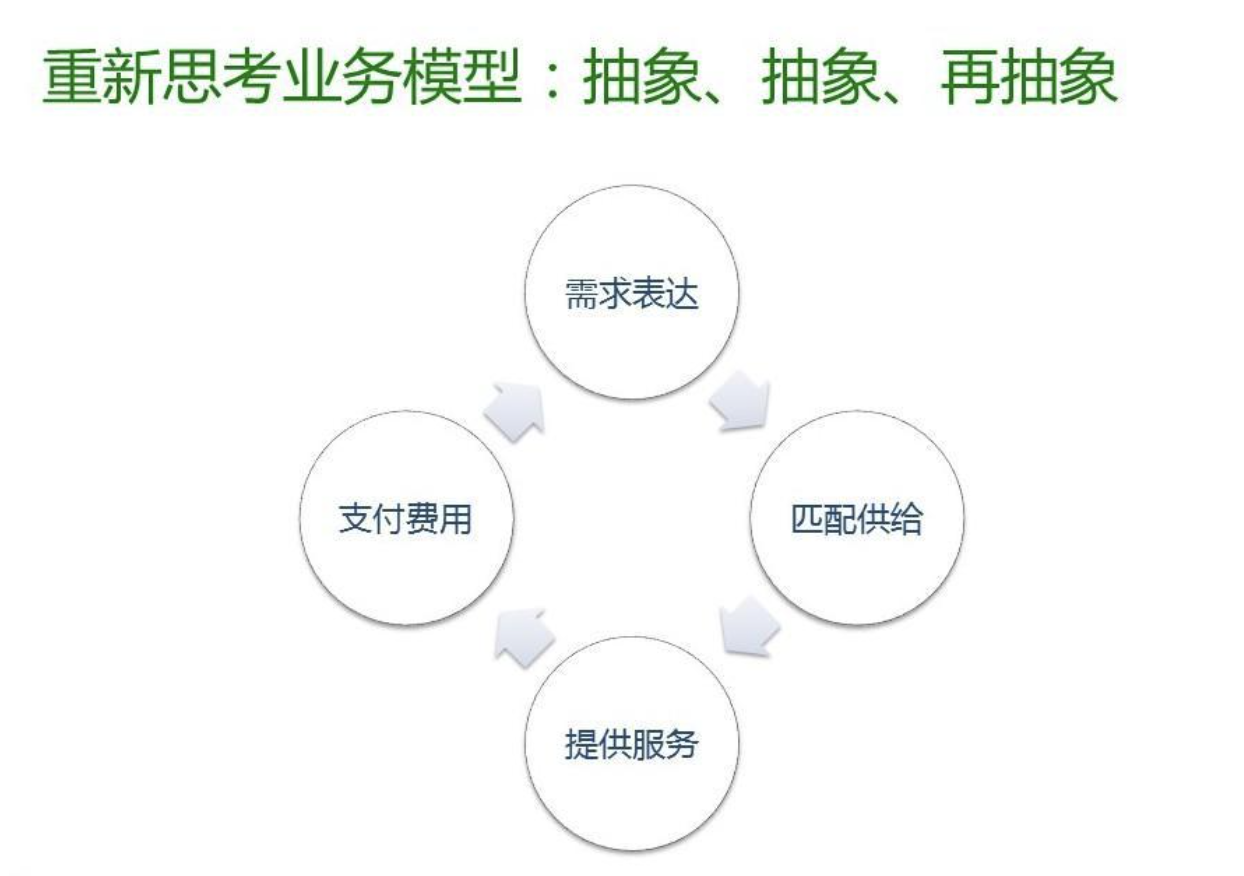
\includegraphics[width=1\textwidth]{fig/DIDI_Reconstruction_21.png}
\end{figure}

\begin{figure}[H]
    \centering
    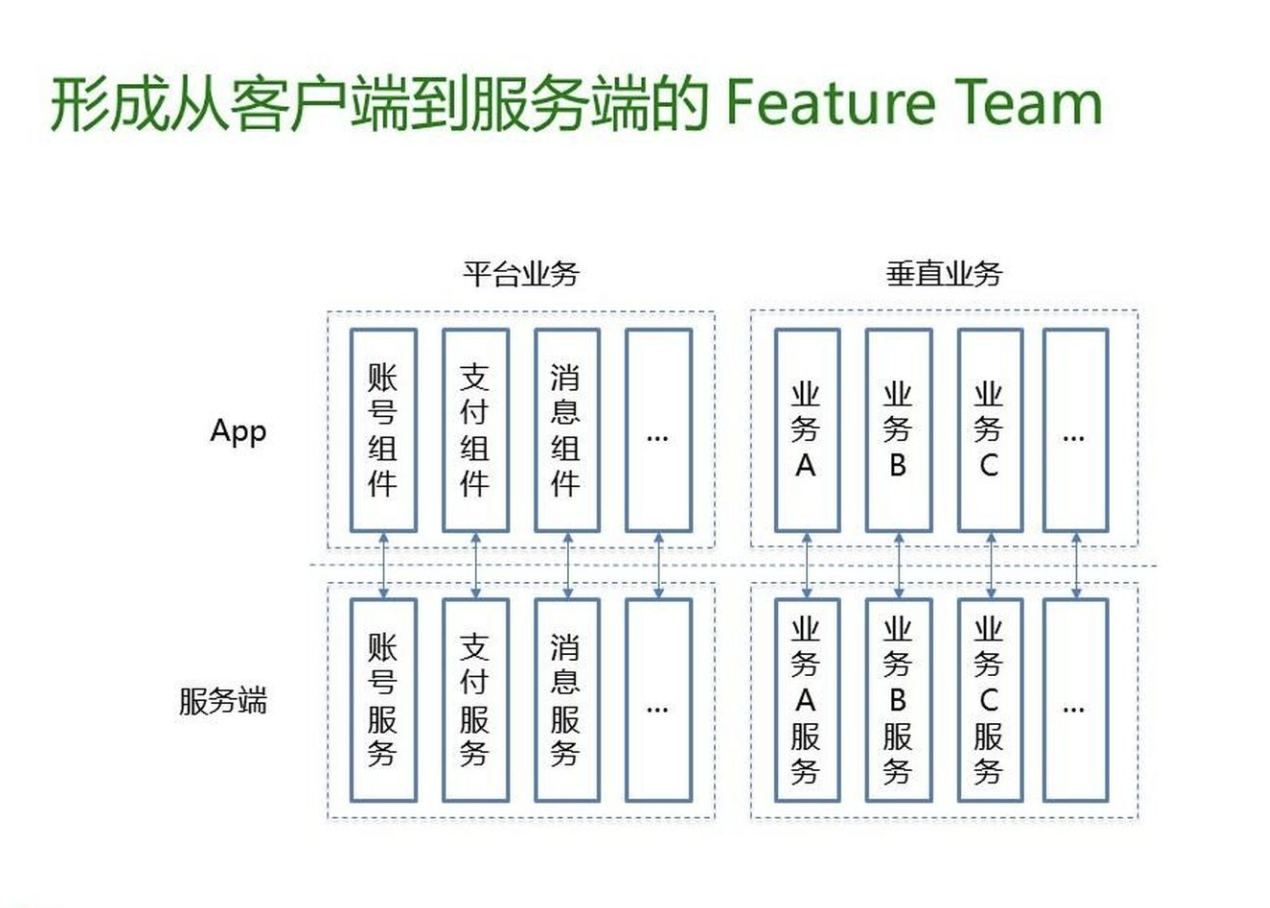
\includegraphics[width=1\textwidth]{fig/DIDI_Reconstruction_22.png}
\end{figure}


另外给大家介绍一下,我们专门做了一个组件平台,叫做魔方组件库,是客户端到服务端的库,我们会继续沉淀更多的客户端到服务端打通的组件,让业务开发更快更轻松。



%\printbibliography
\bibliography{../ref}
\bibliographystyle{IEEEtran}
\end{document}